\part{Fundamentos y el principio de inducción}

\section{Métodos de trabajo en la ciencia}

La forma de trabajo depende de la ciencia que se considere:

\begin{itemize}
	\item En las ciencias experimentales se realizan \textbf{experimentos prácticos} y, a partir de resultados particulares obtenidos en ellos, se extraen resultados generales. Esto se llama \textbf{método inductivo}.
	\item En matematicas, se fijan unos axiomas, se definen unos objetos de trabajo (definiciones) y se combinan axiomas para obtener nuevos resultados llamados teoremas. Esto se denomina \textbf{método deductivo} (se parte de lo general a lo particular). Sus elementos son: \begin{itemize}
		      \item Un axioma es una afirmación cuya veracidad no se cuestiona y en la que se basan el resto de afirmaciones.
		      \item Una definición es una exposición rigurosa de un concepto y sus propiedades que lo diferencian de otros.
		      \item Un teorema es un resultado que se deduce, a través de la lógica, de los axiomas y otros teoremas. A continuación delteorema debe aparecer su demostración (si se cumple la hipotesis, deducimos que obligatoriamente se cumple la tesis). Un ejemplo es el siguiente:
		            \begin{theorem}[de Pitagoras]
			            Si tenemos un triangulo rectangulo cuyos catetos miden \(a \) y \(b \) y la hipotenusa mide \(c \), entonces \(a^{2} + b^{2} = c^{2}   \)
		            \end{theorem}
		      \item Un teorema sin demostracion no es un teorema, sino una conjetura (ejemplo: Conjetura de Goldbach (1742))
	      \end{itemize}
\end{itemize}

\section{Técnicas de demostración}

\subsection{Demostracion directa}
La \textbf{demostración directa} consiste en probar la tesis directamente a partir de la hipótesis.

\begin{theorem}
	Si \(n \) es un numero entero \(n \geq  1\), entonces \(n^{2 } + n \) es par.
\end{theorem}
\begin{proof}
	Si \(n \) es un numero entero \(n \geq  1 \), hay dos casos:
	\begin{enumerate}
		\item Si \(n \) es par, se puede expresar como \(n =2m \) con \(m \in  \Z \). Así, tenemos:
		      \[
			      n^{2} + n = (2m)^{2} + 2m  = 4m^{2} + 2m = \underbrace{2(2m^{2}+m)}_{\text{numero par} }
		      \]
		\item Si \(n \) es impar, se puede expresar como \(n = 2m +1 \) con \(m \in  \Z \). Así,
		      \begin{multline*}
			      n^{2} + n = (2m + 1 )^{2} + (2m+1 ) = 4m^{2} + 4m + 1 + 2m + 1 = \\= 4m^{2} + 6m + 2 = \underbrace{2(2m^{2} + 3m + 1)}_{\text{numero par} }
		      \end{multline*}
	\end{enumerate}
\end{proof}

\subsection{Demostración por contraposición}

Si queremos demostrar por contrarreciproco el teorema \(A \implies B \)  basta con demostrar el teorema \(\neg B \Rightarrow \neg A \) generalmente usando la técnica de demostración directa. Es decir, probamos que lo contrario de la tesis implica lo contrario de la hipótesis.

\begin{theorem}
	Si \(n \) es un numero entero de forma que \(n^{2 } \) es impar, entonces \(n \) es impar.
\end{theorem}
\begin{proof}
	Lo demostraremos por contraposición.

	Supongamos que \(n  \) es un número par. Entonces \(n = 2c, \, c \in \Z\). Sustituyendo,
	\[
		n^{2} = (2c)^{2} = 4c^{2} = 2(2c^{2})
	\]
	Luego \(n^{2} \) también es un número par. Como \(\neg B \Rightarrow \neg A \), se cumple el teorema que queríamos demostrar.
\end{proof}

\subsection{Demostracion por reduccion al absurdo}

Si queremos demostrar por reduccion al absurdo el teorema \(A \Rightarrow B \) basta con que supongamos que se cumpla la hipotesis \((A)\) y lo contrario de la tesis (no B). Si suponemos que se cumple a la vez \(A \) y no \(B\) haciendo deducciones llegamos a que algo es imposible.

\begin{theorem}
	Si \(n \) es un numero entero de forma que \(n^{2} \) es par, entonces \(n \) es par.
\end{theorem}
\begin{proof}
	Lo demostraremos por reduccion al absurdo. Supongamos que se cumple que \(n^{2} \) es par y \(n \) es impar.

	Como \(n \) es impar, entonces \(n = 2c + 1, \; c \in \Z\) y llegamos a
	\[
		n^{2} = (2c+1)^{2} = 4c^{2} + 4c + 1 = \underbrace{2(2c^{2} + c) + 1}_{\text{numero impar} }
	\]
	Luego \(n^{2} \) es impar, pero por hipótesis hemos supuesto que \(n^{2 } \) es par. Ningún número es impar y par a la vez, por lo que hemos llegado a una contradiccion.

	Así tenemos que, si se cumple que \(n^{2} \) es par, entonces obligatoriamente se cumple que \(n \) es par.
\end{proof}

\begin{theorem}
	\label{infinitosprimos}
	Existe una cantidad infinita de numeros primos.
\end{theorem}

\begin{proof}
	En primer lugar, reescribimos el teorema: Si \(A \) es el conjunto de todos los numeros primos, entonces su cardinal es infinito.

	Lo demostramos por reduccion al absurdo. Suponemos que \(A \) es el conjunto de todos los numeros primos y que este conjunto es finito.

	Como \(A \) es finito el conjunto de todos los numeros primos es \(A = \set{p_1,p_2,\ldots,p_n}\). Ahora tomamos
	\[
		x = 1 + p_1 p_2 \cdot \ldots \cdot p_n
	\]
	\(x \) es un numero entero (suma y producto de numeros enteros) y no puede ser un numero primo porque es mayor que todos los numeros que pertenecen a \(A \) ya que si tomamos \(p_j \) en \(A \):
	\[x = 1 + \underbrace{p_1 p_2}_{\geq 1} \cdot \ldots \cdot p_j \cdot \ldots \cdot \underbrace{p_n}_{\geq 1} \geq 1 + p_j > p_j\]
	Ademas, \(x\) no es divisible por ninguno de los primos. Supongamos que \(x \) es divisible por \(p_1\). Entonces \[x = c p_1 = 1 + p_1 p_2 \cdots p_n \Rightarrow 1 = c p_1 - p_1 p_2 \cdots p_n = p_1 (c - p_2 \cdots p_n )\]
	Por tanto, 1 es múltiplo de \(p_1 \). Esto es imposible, pues el \(1 \) solo es múltiplo de si mismo. Esto se repite para el resto de los numeros del conjunto \(A \).

	Es decir, \(x \) es un numero entero que no es primo y tampoco es divisible por ningun numero primo. Como es imposible, llegamos a que el conjunto de los numeros primos no puede ser finito.
\end{proof}

\subsection{Contraejemplos}

Los \textbf{contraejemplos} no son un método de demostración, sino una técnica para demostrar que un teorema es falso.

Basta con encontrar un caso particular (contraejemplo) en el que se cumplen las hipotesis pero no la tesis para probar que el teorema es falso.

\begin{example}
	Pierre de Fermat conjeturó en 1650 que todos los numeros de la forma \(F_n = 2^{2^{n} } + 1 \) son primos, cosa que es cierta si \(n =0,1,2,3\) y \(4 \), pero Leonard Euler demostró que si \(n=5\), el numero resultante no es primo. Asi, se demostró que la conjetura anterior era falsa.
\end{example}

\section{El principio de inducción matemática}
La induccion es un metodo de demostracion basado en uno de los axiomas de los numeros naturales:
\begin{proposition}[Principio de induccion]
	Si \(P \) es una propiedad de forma que se cumple simultaneamente:
	\begin{itemize}
		\item el numero \(n = 1 \) cumple la propiedad \(P \).
		\item siempre que un cierto numero \(n \in \N \) cumple la propiedad \(P\), el siguiente numero \((n+1 )\) también cumple la propiedad \(P \).
	\end{itemize}
	entonces todos los numeros naturales cumplen la propiedad \(P \).
\end{proposition}

Este principio nos da una técnica para probar que un teorema es cierto para todos los numeros naturales, que basta con seguir los siguientes pasos:
\begin{enumerate}
	\item Comprobar que el resultado es cierto para \(n = 1\).
	\item Suponiendo que el resultado es cierto para un numero natural \(n \) (se suele llamar <<hipotesis de induccion>>), demostramos que necesariamente el resultado tambien es cierto para \(n + 1\).
\end{enumerate}

Veamos un ejemplo:
\begin{theorem}
	Demostrar que para cualquier numero natural \(n \in \N \) se cumple que
	\[
		1 + 2 + 3 + \cdots + n = \frac{n(n+1)}{2}
	\]
\end{theorem}
\begin{proof}
	Lo demostraremos por induccion sobre \(n\) . En primer lugar, veamos que se cumple para \(n = 1\).
	\[
		1 + 2 + 3 + \cdots + n \overset{n=1}{=} 1 = \frac{1(1+1)}{2} = \frac{n(n+1)}{2}
	\]
	Suponiendo que es cierto para \(n\), tenemos que demostrar que entonces es cierto para \(n + 1\) y que \(1 + 2 + \cdots + n + (n+1) = \frac{(n+1)(n+2)}{2}\)
	\begin{multline*}
		1 + 2 + 3 + \cdots + n + (n+1) = \frac{n(n+1)}{2} + (n+1) = \\
		= \frac{n(n+1)+2(n+1)}{2} = \boxed{\frac{(n+1)(n+2)}{2}}
	\end{multline*}
\end{proof}

\begin{definition}[Sumatorio y productorio]
	En las formulas relacionadas con sumas o productos de una sucesion de numeros, se utiliza una notacion especial para evitar ambiguedades: los sumatorios y productos. Esta notacion usa dos letras griegas mayusculas: sigma y pi.
\end{definition}
\begin{enumerate}
	\item Si queremos denotar la suma \(a_1 + a_2 + \cdots + a_n \), en lugar de los puntos suspensivos escribimos
	      \[
		      \sum_{i=1}^{n} a_i
	      \]
	      Esta expresion quiere decir que sumamos los elementos de la sucesion \((a_i )\) donde \(i \) recorre todos los valores enteros entre \(i = 1 \) e \(i = n \).
	\item Si queremos denotar el producto \(a_1 \cdot a_2 \cdot \ldots \cdot  a_n \) en lugar de los puntos suspensivos escribiremos
	      \[
		      \prod\limits_{i=1}^{n } a_i.
	      \]
	      Esta expresion quiere decir que multiplicamos los elementos de la sucesion \((a_i )\) donde \(i \) recorre todos los valores enteros entre \(i = 1\) e \(i = n \).

	      Un ejemplo es el factorial de \( n \):
	      \[
		      \prod\limits_{i =1}^{n} i = 1 \cdot 2 \cdot \ldots \cdot n = n!
	      \]
\end{enumerate}

\begin{example}
	Demostrar que para todo \(n \in  \N \) se cumple que
	\[
		\sum_{i=1}^{n} \frac{1}{k(k+1)} = \frac{n}{n+1}
	\]
\end{example}
\begin{proof}
	Lo demostraremos por induccion sobre \(n \). En primer lugar, comprobamos si se cumple para \(n = 1 \).
	\[
		\begin{rcases}
			\sum_{k =1}^{n } \frac{1}{k(k+1)} = \sum_{k=1}^{1} \frac{1}{k(k+1)} =\frac{1}{1(1+1)} = \frac{1}{2} \\
			\frac{n }{n+1 } = \frac{1}{1+1} = \frac{1}{2}
		\end{rcases} \Rightarrow \text{ Cierto para } n = 1
	\]
	Ahora, demostramos que si es cierto para \(n \) entonces también es cierto para \(n + 1 \).

	La hipotesis de induccion es: \(\displaystyle \sum_{k=1}^{n} \frac{1}{k(k+1)} = \frac{n}{n+1}\).

	La tesis de induccion es: \(\displaystyle \sum_{k=1}^{n+1} \frac{1}{k(k+1)}  = \frac{n+1}{n+2} \).

	\begin{multline*}
		\sum_{k=1}^{n+1} \frac{1}{k(k+1)} = \sum_{k=1}^{n } \frac{1}{k(k+1 )} + \frac{1}{(n+1)(n+2)} = \frac{n }{n+1 } + \\ +  \frac{1}{(n+1)(n+2)}
		= \frac{n(n+2) + 1 }{(n+1)(n+2)} = \frac{n^{2} + 2n + 1 }{(n+1)(n+2)} = \\  = \frac{(n+1)^{2}}{(n+1)(n+2)} = \frac{n + 1}{n + 2}
	\end{multline*}
	Asi, llegamos a que tambien se cumple para \(n+ 1\). Luego el principio de induccion es cierto para todo \( n \in  \N \).
\end{proof}

\begin{example}
	Probar que si tenemos \(r \neq  1 \) y \(n \in  \N  \) cualesquiera, entonces
	\[
		1 + r + r^{2} + \cdots + r^{n} = \sum_{j=0}^{n } r^{j}  = \frac{r^{n+1 } - 1 }{r - 1}
	\]
\end{example}
\begin{proof}
	Lo demostraremos por induccion sobre \(n \) (numero natural). Para ello, comprobamos primero si se cumple para \(n = 1\).
	\[
		\sum_{j=0}^{n} r^{j } \overset{n=1}{=} \sum_{j=0}^{1} = 1 + r
	\]
	Por otro lado,
	\[
		\frac{r^{n+1}-1 }{r-1} = \frac{r^{2} - 1 }{r - 1} = \frac{(r+1)(r-1)}{r - 1} = r + 1 = 1 + r
	\]
	Como se cumple para \(n = 1\), supongamos que también se cumple para \(n \) y veamos si es cierto para \(n + 1\): \(\displaystyle \sum_{j=0}^{n+1} r^{j}  = \frac{r^{n+2} - 1 }{r - 1}\).
	\begin{multline*}
		\sum_{j=0}^{n+1} r^{j} = \sum_{j=0}^{n} r^{j} + r^{n+1} = \frac{r^{n+1} -1 }{r-1} + r^{n+1} = \frac{r^{n+1} - 1 + r^{n+1}(r-1)}{r-1} = \\
		= \frac{r^{n+1} - 1 + r^{n+2} - r^{n+1}}{r-1} = \boxed{\frac{r^{n+2} - 1 }{r -1}}.
	\end{multline*}
	Hemos llegado a que la proposicion es cierta para \(n + 1 \). Por tanto, se cumple el principio de induccion para todo \(n \in  \N \) y todo \( r \neq   1\).
\end{proof}

\begin{example}
	Demostrar que para todo \(n \in \N  \) se cumple que \(2^{n} \leq (n+1)! \)
\end{example}
\begin{proof}
	Lo demostraremos por induccion sobre \(n \). En primer lugar, comprobamos si es cierto para \(n = 1 \).
	\[
		2^{n} \leq (n+1)! \Rightarrow 2^{1} \leq (1+1)! = 2 \leq 1 \cdot 2 = 2 \leq 2
	\]
	Como se cumple para \(n = 1 \), supongamos que es cierto para \(n \) y veamos que tambien se cumple para \(n+1 \).

	\[
		2^{n+1} = 2^{n} \cdot 2 \leq (n+1)! \cdot 2
	\]
	Tenemos que probar que \((n+1)! \cdot 2 \leq (n+2)!\)
	\[
		(n+1)! \cdot 2 = 1 \cdot 2 \cdot \ldots \cdot (n+1) \cdot 2
	\]
	\[
		(n+2)! = 1 \cdot 2 \cdot \ldots \cdot (n+1) \cdot (n+2)
	\]
	Como \(2 \leq n +2 \Rightarrow (n+1)! 2 \leq (n+2)!\).

	Entonces, \(2^{n+1} \leq (n+2)! \) y se cumple el teorema para todo \(n \in  \N \).
\end{proof}

\begin{example}
	Probar que si \(n \in  \N \) entonces \(2^{2n} + 5 \) es un multiplo de 3.
\end{example}
\begin{proof}
	Lo probaremos por induccion sobre \(n \). En primer lugar, comprobamos si es cierto para \(n = 1\).

	\[
		2^{2n} + 5 \overset{n=1}{=} 2^{2} + 5 = 4 + 5 = 9 \Rightarrow \text{ multiplo de 3 }
	\]

	Ahora, tendremos que demostrar que si es cierto para \(n \) entonces es cierto para \(n + 1 \).

	Hipotesis de induccion: \(2^{2n} + 5 \) es multiplo de 3.

	Tesis de induccion: \(2^{2(n+1)} + 5\) es multiplo de 3.

	En este caso:
	\begin{multline*}
		2^{2(n+1)} + 5 = 2^{2n + 2} + 5 = 2^{2n} \cdot 2^{2} + 5 = 2^{2n} \cdot 4 + 5 = (2^{2n} + 5 ) + 2^{2n} \cdot 3 = \\
		= 3 \cdot 2^{n} + 3q = \underbrace{3(2^{2n} + q)}_{\text{multiplo de 3}}
	\end{multline*}
	Por tanto, por el principio de induccion la formula es valida para todo \(n \in  \N \).
\end{proof}

\section{Extensiones del metodo de induccion matematica}

Para probar algunas propiedades relacionadas con numeros enteros y subconjuntos de numeros naturales debemos emplear algunas extensiones del Principio de Induccion, como por ejemplo:

\begin{enumerate}
	\item Si queremos probar que una cierta propiedad es valida para todo numero natural \(n \geq  n_0\) (siendo \(n_0 \) un numero natural fijo) usando el principio de induccion, debemos seguir los siguientes pasos: \begin{enumerate}
		      \item Comprobar que el resultado es cierto para \(n = n_0 \).
		      \item Suponiendo que el resultado es cierto para un numero natural \(n \geq n_0 \), demostramos que necesariamente el resultado tambien es cierto para \(n + 1 \).
	      \end{enumerate}
	      Una vez probado esto, habremos demostrado que el resultado es cierto para todo numero natural \(n \geq  n_0 \).

	\item Si queremos probar que una cierta propiedades valida para todo numero entero \(n \in  \Z \) usando el principio de induccion, debemos seguir los siguientes pasos:
	      \begin{enumerate}
		      \item Comprobar que el resultado es cierto para \(n = 0 \).
		      \item Suponiendo que el resultado es cierto para un numero natural \(n \), demostramos que necesariamente el resultado tambien es cierto para \(n + 1 \).
		      \item Suponiendo que el resultado es cierto para un numero entero negativo \(n \leq  0 \), demostramos que necesariamente el resultado tambien es cierto para \(n - 1\).
	      \end{enumerate}

\end{enumerate}

\begin{example}
	Demostrar que si \(n \in  \Z \) entonces \(n^{3} - n \) es multiplo de 3.
\end{example}
\begin{proof}
	Lo demostraremos por induccion sobre \(n \in \Z\). Para ello, primero probamos que se cumple para \(n = 0\).

	\[
		n^{3} - n = 0^{3} - 0 = 0 = 3 \cdot 0 \Rightarrow \text{Es multiplo de 3.}
	\]
	Ahora, comprobamos que si vale para \(n \) entonces tambien vale para \(n + 1 \).
	\begin{multline*}
		(n+1)^{3} - (n+1) = n^{3} + 3n^{2} + 3n + 1 - n - 1 = n^{3} - n + 3n^{2} + 3n \overset{\text{H.I.} }{=} \\
		= 3q + 3n^{2} + 3n = 3(q + n^{2} + n) \Rightarrow \text{Es multiplo de 3. }
	\end{multline*}
	Por ultimo, demostramos que si es cierto para \(n\) entonces tambien lo es para \(n - 1 \).
	\begin{multline*}
		(n-1)^{3} - (n-1) = n^{3} - 3n^{2} + 3n - 1 - n + 1 = n^{3} - n - 3n^{2} + 3n \overset{\text{H.I.}}{=} \\ =  3q - 3n^{2} + 3n = 3(q - n^{2} + n) \Rightarrow \text{Es multiplo de 3.}
	\end{multline*}
	Por tanto, por el principio de induccion hemos demostrado que se cumple el teorema para todo \(n \in \Z \).
\end{proof}

Existe otra extension que se basa en el siguiente principio que se deduce trivialmente del principio de induccion:
\begin{proposition}[Principio de induccion completa]
	Si \(P \) es una cierta propiedad de forma que se cumple simultaneamente:
	\begin{enumerate}
		\item el numero \(n = 1 \) cumple la propiedad \(P \)  y
		\item siempre que un cierto numero \(n \in  \N \) de forma que todos los numeros menores o iguales que el cumple la propiedad \(P \), el siguiente numero tambien cumple la propiedad \(P \)
	\end{enumerate}
	entonces todos los numeros naturales cumplen la propiedad \(P \).
\end{proposition}

\begin{example}
	\label{tfundaritmetica}
	Vamos a demostrar el teorema fundamental de la aritmetica, que dice que todo numero natural \(n > 1 \) puede expresarse (de forma unica) como producto de potencias de numeros primos, es decir
	\[
		n = p^{e_1}_1 \cdot p^{e_2}_2 \cdot \ldots \cdot p^{e_k}_k
	\]
	donde \(k \in \N \), \(p_1, \ldots, p_k \) son numeros primos y \(e_1, \ldots, e_k \in \N \).
\end{example}
\begin{proof}
	Lo demostramos por induccion completa sobre \(n \). Para ello, primero comprobamos que el resultado es cierto para \(n = 2\).

	Como 2 es numero primo, se puede expresar como \(2 = 2^{1}\).

	En segundo lugar, demostramos que si \(1,2,3,\ldots,n \) cumplen la propiedad, entonces \(n + 1 \) cumple la propiedad. Para verlo, hay dos casos:
	\begin{enumerate}
		\item Si \(n + 1\) es primo, entonces \(n + 1 = (n+1)^{1} \; (p_1 = n + 1, \, e_1 = 1 ) \). Cumple la tesis de induccion.
		\item Si \((n+1 )\) no es primo, entonces  es divisible por algun numero menor que \(n + 1 \), luego \(n + 1 = s \cdot t \) con \(s,t \) numeros enteros entre 1 y \(n\).

		      Como \(s\) y \(t \) son numeros enteros entre 1 y \(n \), usando la hipotesis de induccion \(s = p^{e_1}_1 \cdot \ldots \cdot p^{e_k}_k\) y \(t = q^{f_1}_1 \cdot \ldots \cdot q^{f_n}_n  \). Por tanto,
		      \[
			      n + 1 = s \cdot t = \underbrace{p^{e_1}_1 \cdot \ldots \cdot p^{e_k}_k \cdot q^{f_1}_1 \cdot \ldots \cdot q^{f_n}_n}_{\text{Producto de potencias de primos}}
		      \]
	\end{enumerate}
	La unicidad está demostrada en \ref{unicidadtfund}.
\end{proof}
% HACER PROBLEMAS 8, 10, 11, 18, 22, 26, 27, 36 PARA EL VIERNES.

\begin{example}
	Ejercicio 8 - Probar que la suma de los cubos de tres numeros naturales consecutivos es multiplo de 9.
\end{example}
\begin{proof}
	Debemos probar que \(n^{3} + (n+1)^{3} + (n+2)^{3}\) es multiplo de 9 para todo \(n \in \N \). Lo demostraremos por induccion sobre \(n \).

	En primer lugar, comprobamos que es cierto para \(n = 1\).

	\[
		n^{3} + (n+1 )^{3} + (n+2)^{3} = 1^{3} + 2^{3} + 3^{3} = 1 + 8 + 27 = 36 = 9 \cdot 4
	\]
	Ahora, demostramos que si es cierto para \(n \) es cierto para \(n + 1 \).
	\begin{multline*}
		(n+1)^{3} + (n+2)^{3} + (n+3)^{3} = (n+1)^{3} + (n+2)^{3} + (n^{3} + 9n^{2} + 27n + 27) = \\  = n^{3} + (n+1)^{3} + (n+2)^{3} + 9n^{2} + 27n + 27 = 9k + 9n^{2} + 27n + 27 = \\ = \boxed{9(k + n^{2} + 3n + 3)}
	\end{multline*}
	Por el principio de induccion, se cumple para todo \(n \in \N \).
\end{proof}

\part{Combinatoria}
\section{Principios basicos}
\begin{proposition}[Principio del producto]
	Sea \(\mathcal{\MakeUppercase{a}}\) una actividad que se puede realizar en \(t \geq  2 \) pasos secuenciales, de manera que el paso 1 se puede hacer de \(n_1 \) fofrmas distintas, el paso 2 se puede hacer de \(n_2 \) formas distintas, \dots, y el paso \(t \) se puede hacer de \(n_t \) formas distintas.

	Entonces el numero de posibles formas de realizar la actividad \(\mathcal{\MakeUppercase{a}} \) es \(n_1 \cdot n_2 \cdots n_t\).
\end{proposition}

\begin{example}
	Sean \(B_1, B_2, \ldots, B_t \) conjuntos finitos no vacios.

	Calcula \(|B_1 \times B_2 \times \cdots \times B_t|\).

	\(B_1 \times B_2 \times \cdots \times B_t = \set{(b_1, b_2, \ldots, b_t) \mid \forall b_i \exists B_i}\).

	Por tanto, habra \(|B_1| \) opciones de la primera coordenada, \(|B_2| \) opciones de la segunda, \dots, \(|B_t| \) opciones de la t-esima.

	\(|B_1 \times B_2 \times \cdots \times B_t| = B_1 \cdot B_2 \cdots B_t\).
\end{example}

\begin{example}
	El alfabeto español consta de 27 letras de las cuales 5 son vocales. Cuantas palabras (con o sin sentido) de 7 letras se pueden formar de manera que empiecen por vocal y que nunca tengan dos vocales ni dos consonantes seguidas?

	Solucion: se pueden formar \(5^{4} \cdot 22^{3}\) palabras.
\end{example}

\begin{example}
	Se lanzan simultaneamente dos dados de 6 caras, uno de color rojo y otro de color azul. Despues se suman los resultados. De cuantas formas se puede obtener un resultado total de 10 o mas?

	Consideramos varios casos dependiendo de la suma de los dos dados:
	\begin{itemize}
		\item Caso 1: suma 12. Se puede sacar con un 6 en ambos dados (1 forma).
		\item Caso 2: suma 11. Se puede sacar un 6 en el rojo y 5 en el azul o 6 en el azul y 5 en el rojo (2 formas).
		\item Caso 3: suma 10. 5 rojo y 5 azul, 4 rojo y 6 azul, 6 rojo y 4 azul (3 formas).
	\end{itemize}

	La solucion es \(1 + 2 + 3 = 6 \) formas de obtener 10 o mas.
\end{example}

\begin{proposition}
	Sea \(\mathcal{\MakeUppercase{a}} \) una actividad tal que las distintas formas de realizarla son los elementos de un conjunto finito \(B \). Supongamos que \(B \) se puede escribir como union de subconjuntos disjuntos dos a dos, es decir,
	\[
		B = B_1 \cup B_2 \cup \cdots \cup B_t \text{, y si } i \neq j \text{ entonces } B_i \cap B_j = \varnothing
	\]
	Supongamos tambien que \(|B_j| = n_j \).

	Entonces el numero de posibles formas de realizar la actividad \(\mathcal{\MakeUppercase{a}} \) es \(n_1 + n_2 + \cdots + n_t\).

	(Es decir, \(|B| = |B_1 \cup B_2 \cup \cdots \cup B_t| = |B_1| + |B_2| + \cdots + |B_t| \)).
\end{proposition}

\begin{example}
	El alfabeto español consta de 27 letras de las cuales 5 son vocales. Cuantas palabras de 4 letras se pueden formar de manera que empiecen por ``D'' y acaben en consonante o que empiecen por ``F'' y acaben en vocal?

	\begin{itemize}
		\item Caso 1: \(1 \cdot 27^{2} \cdot 22\).
		\item Caso 2: \(1 \cdot 27^{2} \cdot 5\).
	\end{itemize}
	Todos los casos posibles son \(27^{2} \cdot 22 + 27^{2} \cdot 5 = 27^{3} \) (como son casos disjuntos puedo aplicar la regla de la suma).
\end{example}

\begin{example}
	Cuantas palabras de 4 letras se pueden formar de manera que empiecen por ``D'' o acaben en ``F''?

	\begin{itemize}
		\item Caso 1: \(1 \cdot 27^{3}\)
		\item Caso 2: \(1 \cdot 27^{3 } \)
	\end{itemize}
	En este caso, no son disjuntos (por ejemplo, DEEF esta en ambos).

	Debemos restar la interseccion, que será \(1 \cdot 27^{2} \cdot 1 = 27^{2}  \).

	La solucion final es \(27^{3} + 27^{3} - 27^{2}\).
\end{example}

\begin{theorem}
	Sean \(B, B_1, B_2 \) conjuntos finitos tales que \(B= B_1 \cup B_2 \). Entonces
	\[
		|B| = |B_1| + |B_2| - |B_1 \cap B_2|.
	\]
\end{theorem}
\begin{proof}
	Trivial.
\end{proof}

\begin{example}
	Se lanzan dos dados de 6 caras, uno rojo y otro azul. Despues se suman los resultados. De cuantas formas se puede obtener un resultado total de 4 o mas?

	Lo contrario de sacar \(\geq  4 \) es sacar \(< 4 \), que es lo mismo que sacar \(2 \) o \(3 \).

	Para que sume 2, el azul sera 1 y el rojo 1 (1 forma).

	Para que sume 3, hay dos posibilidades: azul 1 y rojo 2, azul 2 y rojo 1.

	En total, hay 4 formas. Podemos sacar el numero de opciones de \(\geq  4 \) restando del total (\(6 \cdot 6 = 36\)). \(36 - 3 = 33 \).
\end{example}

\begin{proposition}[Principio del complementario]
	Sea \(\mathcal{\MakeUppercase{a}} \) una actividad tal que las distintas formas de realizarla son los elementos de un conjunto finito \(B\). Supongamos que \(D \) es otro conjunto finito tal que \(B \subseteq D \) y sabemos que \(|D| = n \) y que \(|D \setminus B| = m\).

	Entonces el numero de posibles formas de realizar la actividad \(\mathcal{\MakeUppercase{a}} \) es \(n - m \). Es decir, \(|B| = |D| - |D \setminus B| \).
\end{proposition}
\begin{remark}
	El principio del complementario es un corolario del principio de la suma.
	\[
		|B| + |D \setminus B| = |D| \Rightarrow |B| = |D| - |D \setminus B|.
	\]
\end{remark}

\begin{example}
	Cuantas palabras de 6 letras se pueden formar de manera que contengan al menos una vocal?

	Como tiene que haber \(\geq  1 \) vocales, lo contrario es que no haya ninguna vocal, que es lo mismo que ``todo consonantes''. En ese caso, hay \(22^{6}\) posibilidades y el total es \(27^{6} \).

	La solucion sera \(27^{6} - 22^{6} \).
\end{example}

\section{Estructuras combinatorias}
\begin{definition}[Variacion con repeticion]
	Una variacion con repeticion de \(m \) elementos \(a_1, a_2, \ldots, a_{m }\) tomados de \(k \) en \(k \) es una lista ordenada formada por \(k \) elementos (que pueden estar repetidos) elegidos cada uno de ellos entre \(a_1, a_2, \ldots, a_m \).

	Denotamos como \(VR_{m,k}\) al numero de variaciones con repeticion de \(m \) elementos tomados de \(k \) en \(k \).
\end{definition}

\vspace{2cm}
\begin{theorem}
	Sean \(m,k \in \N \). Entonces
	\[
		VR_{m,k} = m^{k}.
	\]
\end{theorem}
\begin{proof}
	Aplicacion inmediata de la regla del producto.
\end{proof}

En las variaciones con repeticion importa el orden de los elementos, puede haber elementos repetidos y es posible \(k < m \) o \(k = m \) o \(k > m \).

\begin{example}
	En una prueba de maraton participan 84 corredores. Se otorga una medalla de oro al primero, una de plata al segundo y una de bronce al tercero. De cuantas formas diferentes pueden quedar repartidas las medallas entre los 84 participantes?

	Para el oro, tenemos 84 opciones. Para la plata, hay 83 opciones al no poder repetirse. Para el bronce, hay 82.

	Por tanto, la solucion sera \(84 \cdot 83 \cdot 82 \). Difiere con los ejemplos anteriores al no poder haber repeticiones.
\end{example}

\begin{definition}
	Una variacion de \(m \) elementos \(a_1,a_{2}, \ldots, a_m \) tomados de \(k \) en \(k \) es una lista ordenada formada por \(k \) elementos distintos elegidos cada uno de ellos entre \(a_1,a_2,\ldots,a_m \).

	Denotamos como \(V_{m,k} \) al numero de variaciones de \(m \) elementos tomados de \(k \) en \(k \).

	\[
		V_{m,k} = \prod\limits_{j=m-k+1}^{n } j
	\]
\end{definition}

\begin{definition}
	Sea \(n \in \N \). Se define el factorial de \(n \) como
	\[
		n! \coloneqq \prod\limits_{j=1}^{n } j = n \cdot (n-1) \cdot (n-2) \cdots 3 \cdot 2 \cdot 1.
	\]
	Se define \(0! \coloneqq 1 \).
\end{definition}

\vspace{2cm}
\begin{theorem}
	Sean \(m,k\in  \N\) tales que \(k \leq m \). Entonces
	\(V_{m,k}\) se puede expresar utilizando factoriales:
	\[
		V_{m,k} = \frac{m!}{(m-k)!}
	\]
\end{theorem}

Las variaciones se caracterizan porque importa el orden de los elementos, los elementos son distintos y necesariamente \(k \leq m \).

\begin{example}
	En el problema del maraton quiero decir la clasificacion completa. Es una variacion de 84 elementos tomados de 84 en 84:  \(V_{84,84} = \frac{84!}{(84-84)!}= \frac{84!}{0!} = \frac{84!}{1} = 84!\).
\end{example}

\begin{definition}
	Una permutacion de \(m \) elementos \(a_1,a_2, \ldots, a_m \) es una variacion de esos \(m \) elementos tomados de \(m \) en \(m \).

	Denotamos como \(P_m \) al numero de permutaciones de \(m \) elementos.
\end{definition}

\begin{theorem}
	Sea \(m \in \N \). Entonces:
	\[
		P_m = m!
	\]
\end{theorem}
\begin{proof}
	Es el resultado que se obtiene viendo una permutacion como una variacion.
\end{proof}

\begin{example}
	Cuantas palabras pueden formarse reordenando las letras de la palabra ``murcielago''?

	Es una permutacion de 10 elementos: \(V_{10,10} = P_{10} = 10!\)
\end{example}

En las permutaciones importa el orden de los elementos, los elementos son distintos, son ordenaciones de \(m \) elementos y es un caso particular de variacion con \(m = k \): intervienen todos los elementos.

\vspace{0.2cm}
\begin{example}
	La loteria primitiva es un sorteo en el que se usan todos los numeros consecutivos del 1 al 49. Una apuesta consiste en marcar 6 de esos 49 numeros en un boleto. Cuantas apuestas diferentes existen en la loteria primitiva?

	Si lo hago como una variacion, varias opciones iguales con diferente orden se consideran distintas.

	Cada saco de \(6! \) da una sola apuesta. El numero total de apuestas es el numero total de variaciones dividido entre el numero de variaciones que dan lugar a la misma apuesta:
	\[
		\frac{49 \cdot 48 \cdot 47 \cdot 46 \cdot 45 \cdot 44}{6!} = \frac{V_{49,6}}{P_6} = \frac{\frac{49!}{43!}}{6!} = \frac{49!}{43!6!} = \binom{49}{6}.
	\]
\end{example}

\begin{definition}
	Una combinacion de \(m \) elementos \(a_1,a_2,\ldots,a_m \) tomados de \(k \) en \(k \) es una coleccion no ordenada formada por \(k \) elementos distintos elegidos cada uno de ellos entre \(a_1, a_2, \ldots, a_m \).

	Denotamos como \(C_{m,k}\) al numero de combinaciones de \(m \) elementos tomados de \(k \) en \(k \). Una notacion alternativa para \(C_{m,k}\) es \(\binom{m }{k }\) (numero combinatorio, se lee \(m \) sobre \(k\)).
\end{definition}
\begin{theorem}
	Sean \(m,k \in \N \) tales que \(k \leq m \). Entonces
	\[
		C_{m,k} = \frac{m!}{k! \cdot (m-k)!}
	\]
\end{theorem}
\begin{proof}
	Hay \(V_{m,k} = \frac{m!}{(m-k)!}\) variaciones de \(m \) elementos tomados de \(k \) en \(k \)

	Hay varias variaciones que dan la misma combinacion. ¿Cuantos? \(P_k = k! \) que son las distintas formas de permutar los \(k \) elementos.

	Por tanto, el numero de combinaciones
	\[
		C_{k,m} = \frac{V_{m,k}}{P_k} = \frac{m! }{(m-k)! \cdot k!}
	\]
\end{proof}

En las combinaciones, no importa el orden de los elementos, los elementos son distintos y necesariamente \(k \leq m \).

\begin{example}
	Cuantas palabras pueden formarse reordenando las letras de la palabra ``SOCORRO''?

	No se puede contar como una variacion porque se puede reordenar de forma distinta y de lugar a la misma palabra.

	Para contar contar, vamos a pensar temporalmente que las letras son las 7 distintas. Ahora puedo considerar las permutaciones de estos 7 simbolos distintos: son \(7! \).

	Por ejemplo, cuantas veces va a salir SOOCORR contando como permutaciones de 7 elementos distintos? En este caso, son 12 posibilidades porque hay 3 O y 2 R (\(3! \cdot 2! = 12\)). \(3! \) son las formas de permutar las O y \(2! \) las formas de permutar las R.

	Luego el numero total de palabras que puedo obtener son \(\frac{7! }{3!2!} = P^{3,2}_7 \) (visto en la siguiente definicion).

	Los parametros son el numero total de simbolos y el numero de repeticiones de cada uno (3,2,1,1).

	\(a_1 = O (n_1 = 3), a_2 = R (n_2 = 2), a_3 = S (n_3 = 1), a_4 = C (n_4 = 1)\).
\end{example}

\begin{definition}
	Una permutacion con repeticion de \(n \) elementos \(a_1,a_2, \ldots, a_m \) donde cada \(a_i \) se repite \(n_i \) veces es una lista ordenada de \(n \) elementos elegidos entre \(a_1,a_2,\ldots,a_m \) donde el elemento \(a_i \) aparece repetido \(n_i \) veces.

	Supongamos que \(n_i > 1 \) siempre que \(i \leq k \) y que \(n_i = 1 \) siempre que \(i > k \). Denotamos como \(P^{n_1,n_2,\ldots,n_k}_n \) al numero de permutaciones con repeticion de \(n \) elementos donde hay \(k \) elementos que se repiten \(n_1,n_2, \ldots, n_k \) veces respectivamente.
\end{definition}
\begin{theorem}
	Sea \(n,n_1,n_2,\ldots,n_k \in \N \) tales que \(\sum_{i=1}^{k} n_i \leq n \). Entonces
	\[
		P^{n_1,n_2,\ldots,n_k}_{n} = \frac{n! }{\prod_{i =1}^{k} n_i !} = \frac{n! }{n_1! \cdot n_2! \cdots n_k!}
	\]
\end{theorem}
\begin{proof}
	Extrapolar las ideas del ejemplo que hemos visto. No lo escribimos.
\end{proof}

\begin{example}
	De combinaciones con repeticion. Sabemos que la seleccion olimpica española ha obtenido un resultado final de 10 medallas en los ultimos juegos. De cuantas formas pueden estar distribuidas esas medallas entre oro, plata y bronce?

	Genero 12 huecos (10 para medallas y 2 para separadores que van a separar las medallas de oro de las de plata y las de plata de las de bronce).

	Dos hechos:
	\begin{enumerate}
		\item Hay el mismo numero de medallas posibles que de estructuras con separadores.
		\item La estructura queda totalmente determinada si se conoce la posicion de los dos separadores.
	\end{enumerate}

	De cuantas formas diferentes puedo poner los separadores? Como tengo que elegir los dos huecos para los dos separadores de entre 12 posibles y no importa el orden en el que lo haga:
	\[
		C_{12,2} = \binom{12 }{2 } = \frac{12! }{2!10! } = \frac{12 \cdot 11 }{2}
	\]
	Como seria el caso general?

	Hay \(m \) elementos \(a_1, \ldots, a_m \) (\(n = 3 \)). Hay que elegir \(k \) veces pudiendo repetir (\(k = 10\)).

	Para el mismo argumento, necesitamos \(m - 1 \) separadores. Habra \(k + m - 1 \) huecos.

	De cuantas formas se pueden elegir los huecos de los separadores? \(\binom{k + m - 1}{m - 1 } = \binom{k + m - 1 }{k}\).
\end{example}

\begin{definition}
	Una combinacion con repeticion de \(m \) elementos \(a_1,\ldots,a_m \) tomados de \(k \) en \(k \) es una coleccion no ordenada formada por \(k \) elementos (que pueden estar repetidos) elegidos cada uno de ellos entre \(a_1,\ldots, a_m \).

	Denotamos como \(CR_{m,k}\) al numero de combinaciones de elementos tomados de \(k \) en \(k \).
\end{definition}

\begin{theorem}
	Sean \(m,k \in \N \). Entonces
	\[
		CR_{m,k} = \binom{m+k-1}{m-1} = \frac{(m+k-1)!}{(m-1)! \cdot k!}.
	\]
\end{theorem}

\section{Numeros combinatorios}
\begin{definition}
	Se amplia la definicion de numero combinatorio al caso \(k = 0 \) como
	\[
		\binom{m }{0 } \coloneqq 1.
	\]
\end{definition}

Triangulo de Pascal. El numero de una fila es la suma de los dos numeros superiores.

\begin{theorem}[Simetria del triangulo de Pascal]
	Sean \(m \in \N \), \(k \in \N \cup \set{0}, k \leq m \). Entonces:
	\[
		\binom{m }{k }= \binom{m }{m - k }.
	\]
\end{theorem}
\begin{proof}
	Demostracion analitica con la formula.

	\[\binom{m }{k } = \frac{m! }{(m-k)! k! }\]

	\[
		\binom{m }{m - k } = \frac{m! }{(m - (m-k))! (m-k)! } = \frac{m! }{(m-k)! k! }.
	\]
\end{proof}
\begin{proof}
	Demostracion con combinatoria.

	\[
		\binom{m }{k } = \text{ las formas de elegir } k \text{ elementos de entre } m \text{ posibles.}
	\]
	\[
		\binom{m }{m-k } = \text{ las formas de elegir } m - k \text{ elementos de entre } m \text{ posibles.}
	\]
	Cada eleccion de \(k \) elementos lleva implicita una eleccion de \(m - k \) elementos (el complementario del conjunto elegido). Por tanto, hay las mismas formas de elegir \(k \) elementos que de \(m-  k\). Luego
	\[
		\binom{m }{k } = \binom{m }{m - k }.
	\]
\end{proof}

\begin{theorem}[Calculo iterativo de los numeros combinatorios]
	Sean \(m \in \N \), \(k \in \N \cup \set{0}, k < m \). Entonces:
	\[
		\binom{m+1 }{k + 1 } = \binom{m }{k } + \binom{m }{k + 1 }
	\]
\end{theorem}
\begin{proof}
	Demostracion analitica.

	\begin{multline*}
		\binom{m }{k }+ \binom{m }{k + 1} = \frac{m! }{(m-k)! k! } + \frac{m! }{(m-k-1)! (k+1)! } = \\
		= \frac{m! (k+1)}{(m-k)!k! (k+1)} + \frac{m! (m-k)}{(m-k)(m-k-1)!(k+1)! } = \\
		= \frac{m!(k+1)}{(m-k)!(k+1)!} + \frac{m!(m-k)}{(m-k)!(k+1)!} = \frac{m!(m+1)}{(m-k)!(k+1)!} = \\ = \boxed{\frac{(m+1)!}{(m-k)!(k+1)!}}.
	\end{multline*}
\end{proof}
\begin{proof}
	Demostracion combinatoria. Hecha en clase.
\end{proof}

\begin{theorem}[Binomio de Newton]
	Sean \(a,b \in \R \), \(n \in \N \). Entonces:
	\[
		(a+b)^{n} = \sum_{j =0 }^{n } \binom{n }{j } a^{j} b^{n-j }.
	\]
\end{theorem}
\begin{proof}
	Lo demostraremos por induccion sobre \(n \). En primer lugar, comprobamos si se cumple para \(n = 1 \):
	\[
		\sum_{j =0 }^{1 } \binom{1 }{j } a^{j} b^{1-j } = \binom{1 }{0 } a^{0 } b^{1 } + \binom{1 }{1 } a^{1 } b^{0} = b + a = (a+b)^{1}
	\]
	Suponemos que se cumple para \(n \) y veamos si tambien para \(n + 1 \). Es decir, \((a+b)^{n+1} = \sum_{j =0 }^{n+1 } \binom{n+ 1 }{j } a^{j } b^{n + 1 - j } \) (tesis de induccion).

	\begin{multline*}
		(a+b)^{n+1} = (a+b)^{n} \cdot (a+b) \overset{H.I.}{=} \sum_{j =0 }^{n } \binom{n }{j } a^{j} b^{n-j } \cdot (a+b) = \\
		= a \sum_{j =0 }^{n } a^{j} b^{n-j } + b \sum_{j =0 }^{n } a^{j} b^{n-j } = \sum_{j =0 }^{n } \binom{n }{j }a^{j+1} b^{n-j } + \sum_{j =0 }^{n } \binom{n }{j } a^{j} b^{n-j+1} = \\
		= \binom{n }{n } a^{n+1} b^{0 } + \sum_{j =0 }^{n- 1} \binom{n }{j } a^{j+ 1 } b^{n-j } + \sum_{j =1}^{n }  \binom{n }{j } a^{j } b^{n-j + 1 } + \binom{n }{0} a^{0 }b^{n+1} = \\
		= \binom{n }{n }a^{n+1 } b^{0} + \sum_{j =1 }^{n} \binom{n }{j - 1} a^{j}b^{n-(j-1)} + \sum_{j =1}^{n } \binom{n }{j }a^{j } b^{n-j+1 } + \binom{n }{0 }a^{0 } b^{n+1 } = \\
		= \binom{n }{n }a^{n+1 } b^{0} + \sum_{j =1}^{n } \left (\binom{n }{j - 1 } a^{j } b^{n-(j-1)} + \binom{n }{j } a^{j } b^{n-j+1}\right ) + \binom{n}{0} a^{0 } b^{n+1} =  \\
		= \binom{n }{n }a^{n+1 } b^{0 } + \sum_{j=1}^{n} \left ( \left (\binom{n }{j } + \binom{n }{j - 1} \right ) a^{j }b^{n+1-j}  \right ) + \binom{n }{0 }a^{0 } b^{n+1} = \\
		= \boxed{\sum_{j =0 }^{n+ 1} \binom{n + 1 }{j }a^{j } n^{n+1-j }}.
	\end{multline*}
\end{proof}

\begin{theorem}[Suma de una fila del triangulo de Pascal]
	Sea \(n \in \N \). Entonces:
	\[
		\sum_{j =0 }^{n } \binom{n }{j } = 2^{n }.
	\]
\end{theorem}
\begin{proof}
	Lo demostramos con el binomio de Newton con \(a = 1 \) y \(b = 1 \).
	\[
		(1+1)^{n} = \sum_{j =0 }^{n } \binom{n }{j} 1^{j} 1^{n -j} = \sum_{j =0 }^{n } \binom{n }{j}.
	\]

	Existe una demostracion alternativa al teorema usando combinatoria.

	Supongamos que \(A \) es un conjunto con \(n \) elementos. Si pensamos en todos los subconjuntos posibles de \(A \), sabemos que hay \(2^{n } \) (demostrado en Logica).

	Lo divido en casos:
	\begin{enumerate}
		\item Conjuntos con 0 elementos. \(1 = \binom{n }{0 }\)
		\item Conjuntos con 1 elemento. \(\binom{n }{1 }\)
		\item Conjunto con 2 elementos. \(\binom{n }{2}\)
		\item[n.] Conjunto con n elementos. \(\binom{n }{n }\)
	\end{enumerate}
	Luego \(2^{n }= \binom{n }{0 } + \binom{n}{1 } + \binom{n }{2 } + \cdots + \binom{n }{n }\)
\end{proof}

\part{Aritmética entera y modular}
\section{Divisibilidad en \(\Z \). Algoritmo de Euclides.}
\begin{definition}
	Sea \(\R \) el conjunto de los numeros reales. Dado \(a \in \R \), se define el valor absoluto de \(a \) como
	\[
		|a| \coloneqq \begin{dcases}
			a \text{ si } a \geq 0 \\
			-a \text{ si } a < 0
		\end{dcases}
	\]
\end{definition}

\begin{proposition}
	\(\forall  a,b \in \R \) se cumple
	\begin{enumerate}
		\item \(|a + b| \leq |a| + |b| \) (desigualdad triangular)
		\item \(|a \cdot b | = |a| \cdot |b| \)
	\end{enumerate}
\end{proposition}
\begin{proof}
	Demostrar por nuestra cuenta (facil).
\end{proof}

\begin{definition}[Cotas superiores e inferiores, maximos y minimos]
	Sea \(A \) un conjunto no vacio de una relacion de orden que denotaremos \(\leq \). Sea \(B \subseteq A \).
	\begin{itemize}
		\item \(a \in A \) es cota superior de \(B \) si \(\forall  b \in B \quad b \leq a\).
		\item \(a \in A\) es cota inferior de \(B \) si \(\forall b \in B \quad a \leq b \).
		\item Si \(b \) es una cota superior de \(B \) y ademas \(b \in B \), decimos que \(b \) es el maximo de \(B \).
		\item Si \(b \) es una cota inferior de \(B \) y ademas \(b \in B \), decimos que \(b \) es el minimo de \(B \).
	\end{itemize}
\end{definition}

\begin{example}
	Sea \(\Z = \set{\ldots,-2,-1,0,1,2,\ldots }\) el conjunto de los numeros enteros, dotado de la relacion de orden habitual que denotaremos \(\leq  \).
	\begin{itemize}
		\item \(B = \set{-1,1,3,5} \subseteq \Z \). \begin{itemize}
			      \item \(-8,-5,-4,-1 \) son ejemplos de cotas inferiores de \(B \).
			      \item \(-1 \) es el minimo de \(B \).
			      \item \(5,6,9,43 \) son ejemplos de cotas superiores de \(B \).
			      \item \(5 \) es el maximo de \(B \).
		      \end{itemize}
		\item \(B = \N = \set{1,2,3,4,5,\ldots } \subseteq \Z\) \begin{itemize}
			      \item \(-8,-1,0,1 \) son ejemplos de cotas inferiores de \(B \).
			      \item \(1 \) es el minimo de \(B \).
			      \item \(B \) no esta acotado superiormente.
			      \item \(B \) no tiene maximo.
		      \end{itemize}
	\end{itemize}
\end{example}

\begin{proposition}
	En \(\Z \) se cumple que:
	\begin{itemize}
		\item Todo conjunto no vacio y acotado inferiormente tiene minimo.
		\item Todo conjunto no vacio y acotado superiormente tiene maximo.
	\end{itemize}
\end{proposition}
\begin{proof}
	Obvio.
\end{proof}

\begin{example}
	Este resultado no es cierto en otros conjuntos ordenados. Por ejemplo \(\Q \):
	\begin{itemize}
		\item Sea \(B = (1,3) \cap \Q \coloneqq \set{x \in \Q \mid 1 < x < 3 }\).
		\item \(-3, 0, \frac{1}{2}, 1 \) son ejemplos de cotas inferiores.
		\item \(B \) no tiene minimo. 1 es el infimo de \(B \).
		\item \(3,\frac{8}{3},9,27 \) son ejemplos de cotas superiores.
		\item \(B \) no tiene maximo.
	\end{itemize}
\end{example}

\begin{theorem}[de la división entera]
	Sean \(a,b \in \Z \) con \(b \neq 0 \). Entonces existen \(q,r \in \Z \) que cumplen
	\begin{enumerate}
		\item \(a = bq + r \)
		\item \(0 \leq r \leq |b| \)
	\end{enumerate}
	Ademas \(q \) y \(r \) son los unicos enteros que cumplen simultaneamente las dos condiciones anteriores.
\end{theorem}
\begin{proof}
	No demostrada en clase.
\end{proof}

\begin{example}
	~\begin{enumerate}
		\item \(a = 27, \quad b = 5 \)

		      \(q = 5, \quad r = 2 \)

		      \(0 \leq 2 \leq 5 \)
		\item \(a = -27, \quad b = 5 \)

		      \(q = -5\)

		      \(-27 = (-5) \cdot 5 + (-2) \) X

		      \(-27 = \underbrace{(-6)}_{q} \cdot 5 + \underbrace{3}_{r} \)

		\item \(a = 27, \quad b = -5 \)

		      \(27 = (-5)(-5) + 2 \)

		      \(q = -5, \quad r = 2 \)

		\item \(a = -27, \quad b = -5\)

		      \(-27 = (-5) \cdot 6 + 3 \)

		      \(q = 6, \quad r = 3\)
	\end{enumerate}
\end{example}

\begin{definition}[Divisor, multiplo]
	Sean \(a, b \in \Z \). Decimos que \(b \) es divisor de \(a \) si existe \(q \in \Z \) tal que \(a = bq \).

	Decimos tambien que \(b \) divide a \(a \) o que \(a \) es multiplo de \(b \).

	Notacion: \(a|b\)
\end{definition}

\begin{proposition}[Propiedades de la relacion de divisibilidad]
	\(\forall a,b,c,d,e \in \Z \) se cumple
	\begin{enumerate}
		\item \(a\mid 0 \)
		\item \(a \neq 0 \Rightarrow 0 \nmid a \)
		\item \(a|b, b | c \Rightarrow a|c \)
		\item \(a | a, \;1 | a,\; -a | a, \;-1 | a\)
		\item \(a | b, c| d \Rightarrow ac | bd \)
		\item \(a | b \Rightarrow a | bd \)
		\item \(c \neq 0 \Rightarrow (a|b \iff ac|bc )\)
		\item \(a|b, a|c \Rightarrow a|bd + ce\)
		\item \(a|b, b \neq 0 \Rightarrow |a| \leq |b| \)
		\item \(a|b,b|a \Rightarrow |a| = |b|\)
	\end{enumerate}
\end{proposition}
\begin{proof}
	~\begin{enumerate}
		\item \(\forall  a \in \Z \) \(\; a \mid 0 ?\)

		      \[
			      0 = 0 \cdot a \Rightarrow a \mid 0
		      \]
		\item Supongamos que \(0 \mid a \Rightarrow \exists n \in \Z\) tal que \(a = 0 \cdot n = 0 \), pero tenemos que \(a =  0 \). Hemos llegado a una contradiccion, luego \(0 \nmid a \) (revisar)
		\item \(a \mid b \Rightarrow \exists n \in \Z \) tal que \(b = q \cdot n \)

		      \(b \mid c \Rightarrow \exists m \in \Z \) tal que \(c = b \cdot m \).

		      \(c = b \cdot m = q \cdot n \cdot m \Rightarrow a \mid c \)

		\item \(a = 1 \cdot a \Rightarrow 1| a, a | a\)

		      \(a = (-1)(-a) \Rightarrow -1 \mid a, -a \mid a \)

		\item \(a|b \Rightarrow \exists n \in \Z \) tal que \(b = a \cdot n \)

		      \(c|d \Rightarrow \exists m \in \Z \) tal que \(d = c \cdot m \)

		      \(b \cdot d = a \cdot n \cdot c \cdot m \Rightarrow ac \mid bd \)
		\item \(a|b \Rightarrow a|bd \)

		      Tomo \(c= 1 \) en 5) y obtengo el resultado.
		\item \(c \neq 0\)

		      \begin{enumerate}
			      \item \(a|b \Rightarrow ac | bc \)
			            \[
				            \begin{dcases}
					            a|b \\
					            c|c
				            \end{dcases} \overset{5)}{\Rightarrow} ac|bc
			            \]
			      \item \(ac|bc \Rightarrow \exists m \in \Z \) tal que \(bc = acm \Rightarrow b = a \cdot m \Rightarrow a | b \).
		      \end{enumerate}
		\item \(a | b \Rightarrow \exists m \in \Z \) tal que \(b = a \cdot m \)

		      \(a | c \Rightarrow \exists n \in \Z \) tal que \(c = a \cdot n \)

		      \(bd + ce = a \cdot m \cdot d + a \cdot n \cdot e = a (md + ne) = a (md + ce )\)

		\item \(a|b \Rightarrow \exists m \in \Z \) tal que \(b = a \cdot m \)

		      Tomo valor absoluto: \(|b| = |a \cdot m| = |a| \cdot |m| \geq |a|\)

		      Como \(b \neq 0\), \(m \neq 0 \) y \(|m| \geq  1	\)

		\item Supongamos que \(a|b \) y \(b|a \).
		      \begin{description}
			      \item[Caso 1] Si \(a = b = 0 \Rightarrow |a| = |b|\)
			      \item[Caso 2] Si \(a \neq 0, b \neq 0\)

				      Por 4, \(a|b \Rightarrow |a| \leq |b| \), \(b|a \Rightarrow |b| \leq |a| \). Luego \(|a| = |b|\).

		      \end{description}
		      Obs: no puede pasar \(a = 0, b \neq 0 \) o \(a \neq 0, b = 0 \) por (2).
	\end{enumerate}
\end{proof}

\begin{corollary}
	La relacion de divisibilidad es una relacion de orden parcial en \(\N \).
\end{corollary}

\begin{definition}[Numero primo]
	Sea \(n \in \N, n \geq  2 \). Decimos que \(n \) es primo si sus unicos divisores positivos son \(1 \) y \(n \). En caso contrario decimos que \(n \) es compuesto.
\end{definition}

\begin{theorem}
	Sea \(n \in \N, n \geq 2 \). Se cumple
	\[
		n \text{ es compuesto} \iff  \exists d \text{ divisor de } n \text{ tal que } 2 \leq d \leq \sqrt{n }
	\]
\end{theorem}
\begin{proof}
	\(\Leftarrow )\) Obvio. Si hay algun divisor \(2 \leq d \leq \sqrt{n } \Rightarrow d \neq 1, d \neq n \Rightarrow n\) es compuesto.

	\(\Rightarrow ) \) \(n \text{ compuesto} \Rightarrow \exists d_1 \text{ divisor positivo de } n \text{ tal que } d_1 \neq 1, d_1 \neq n\).

	Como \(d_1 \) es divisor de \(n \Rightarrow \exists d_2 \in \N \) tal que \(n = d_1 \cdot d_2 \).

	Sabemos que \(d_1 \geq  2 \). Tambien \(d_2 \geq  2\) (porque, si no, \(d_1 \) seria \(n\)).

	Lo demostramos por reduccion al absurdo. Supongamos que ambos, tanto \(d_1 \) como \(d_2 \) son mayores que \(\sqrt{n } \):
	\[
		n = d_1 \cdot d_2 > \sqrt{n} \cdot \sqrt{n} = n
	\]
	Esto es una contradiccion. Luego uno de los dos es menor o igual que \(\sqrt{n }\).
\end{proof}

\begin{theorem}[Teorema fundamental de la aritmetica]
	Sea \(n \in \N \), \(n \geq  2 \). Entonces \(n \) se puede escribir de manera unica (salvo el orden de los factores) como producto de factores primos. Mas formalmente:
	\begin{itemize}
		\item Existencia: \(\exists p_1,p_2,\ldots,p_k \) primos tal que \(n = p_1 p_2 \cdots p_k \)
		\item Unicidad: Si \(n = p_1 p_2 \cdots p_k \) y \(n = q_1 q_2 \cdots q_m \) donde los \(p_j \) y \(q_j \) son primos, entonces: \begin{itemize}
			      \item \(k = m\)
			      \item Se pueden reordenar los factores de manera que \(\forall j\; p_j = q_j \)
		      \end{itemize}
	\end{itemize}
\end{theorem}

\begin{proof}
	\label{unicidadtfund}
	La existencia se puede demostrar por induccion completa, como vimos en la demostración \eqref{tfundaritmetica}.

	La unicidad se demuestra más adelante.
\end{proof}

\begin{theorem}
	Hay infinitos numeros primos.
\end{theorem}
\begin{proof}
	Demostrado en \eqref{infinitosprimos}.
\end{proof}

\begin{definition}[Maximo comun divisor]
	Sean \(a,b \in \Z \) con \((a,b) \neq (0,0)\). Se define el maximo comun divisor de \(a \) y \(b \) como el mayor divisor comun positivo de \(a \) y \(b \).

	Notacion: \(\mathrm{m.c.d.}(a,b) \).

	Por definicion se adopta \(\mathrm{m.c.d.}(0,0) \coloneqq 0\).
\end{definition}

\begin{proposition}[Existencia m.c.d]
	\(\forall a,b \in \Z \) existe \(\mathrm{m.c.d.}(a,b) \).
\end{proposition}
\begin{proof}
	Sea \(D = \set{n \in \N \mid n \text{ es divisor comun de } a \text{ y } b }\).

	Supongamos, sin perdida de generalidad, que \(a \neq 0 \). Todos los elementos de \(D \) son \(\leq |a| \).

	Luego \(|a| \) es una cota superior de \(D \). Por tanto \(D \) tiene maximo.

	Ese numero es el maximo comun divisor de \(a \) y \(b \).

	Observacion: Estamos usando que \(D \neq 0 \) porque \(1 \in D \).
\end{proof}

\begin{definition}
	Sean \(a,b \in \Z \). Decimos que \(a \) y \(b \) son relativamente primos entre si o coprimos si \(\mathrm{m.c.d.}(a,b) = 1 \).
\end{definition}

\begin{proposition}
	~\begin{enumerate}
		\item \(\forall a \in \Z \quad \mathrm{m.c.d.}(a,0) = |a| \)
		\item \(\forall a,b \in \Z \quad \mathrm{m.c.d.}(a,b) = \mathrm{m.c.d.}(|a|,|b|) \)
		\item \(\forall a,b \in \N \quad 1 \leq \mathrm{m.c.d.}(a,b) \leq \mathrm{min}(a,b)  \)
	\end{enumerate}
\end{proposition}
\begin{proof}
	~\begin{enumerate}
		\item \(|a| \) es el divisor mas grande de \(a \) y ademas \(|a| \) divide a 0 \(\Rightarrow \mathrm{m.c.d.}(a,0) = |a| \)
		\item Es porque los divisores positivos de \(a \) son los mismos que los divisores positivos de \(b \).
		\item Se debe a que los divisores de un numero positivo son menores o iguales que ese numero.
	\end{enumerate}
\end{proof}

\begin{proposition}
	\label{mcd}
	Sean \(a,b \in \N \). Sea \(r \) el resto de la division entera de \(a \) entre \(b \). Entonces
	\[
		\mathrm{m.c.d.}(a,b) = \mathrm{m.c.d.}(b,r)
	\]
\end{proposition}

\begin{proof}
	\(a,b \in \N \), r es el resto de la division \(a = bq + r \) y \(a < r < b \).

	Vamos a considerar \(D_1 = \set{d_1 \in \N \mid d_1 \text{ es divisor comun de a y b}}\) y \(D_2 = \set{d_2 \in \N \mid d_2 \text{ es divisor comun de b y r}}\).

	Vamos a ver que \(D_1 = D_2 \).

	\(\subseteq )\) Sea \(d \in D_1 \Rightarrow d_1 \) es divisor de \(a \) y \(b \Rightarrow \exists m,n \in \N\) tal que \(a = m \cdot d \) y \(b = n \cdot d \).

	Entonces \(r = a - bq = m \cdot d - n \cdot d \cdot q \Rightarrow d(m - nq) \Rightarrow d | r \)

	Como tambien \(d | b \), \(d \in D_2 \).

	\(\supseteq ) \) Sea \(d \in D_2 \Rightarrow d | b \) y \(d | r  \Rightarrow \exists m,n \in \N\) tal que \(b = d \cdot m, \; r = d \cdot n \).

	Luego \(a = bq + r = d \cdot q + d \cdot r = d (mq + n ) \Rightarrow d | a \). Como tambien \(d | b \), \(d \in D_1 \).

	Como \(D_1 = D_2 \Rightarrow \mathrm{m.c.d.}(a,b) = \mathrm{m.c.d.}(b,r)  \)
\end{proof}

\begin{example}
	Calcular el m.c.d. de 250 y 32.

	\(250 = 32 \cdot 7 + 26 \)

	\(\mathrm{m.c.d.}(250,32) = \mathrm{m.c.d.}(32,26)  \)

	\(32 = 26 \cdot 1 + 6 \)

	\(26 = 6 \cdot 4 + 2 \)

	\(6 = 2 \cdot 3 + 0\)

	\(\mathrm{m.c.d.}(32,26) = \mathrm{m.c.d.}(26,6) = \mathrm{m.c.d.}(2,0) = 2  \)
\end{example}

\begin{theorem}[Algoritmo de Euclides]
	Sean \(a,b \in \N \) con \(a > b \). Consideramos la siguiente sucesion construida recursivamente:
	\begin{itemize}
		\item \(r_0 \coloneqq a \)
		\item \(r_1 \coloneqq b \)
		\item Sea \(k \geq 2 \). Supongamos que ya hemos construido todos los elementos de la sucesion hasta \(r_{k-1}.\) Si \(r_{k-1} > 0 \)  construimos \(r_k \) como el resto de la division entera de \(r_{k-2}\) entre \(r_{k-1}\)

		      (es decir, tal que \(r_{k-2} = r_{k-1}q_k + r_k \) para algun \(q_k \in \N \) y \(0 \leq r_k \leq  r_{k-1}\) )
	\end{itemize}
	Entonces se cumple:
	\begin{itemize}
		\item \(\exists  n \in \N \mid r_n = 0 \)
		\item \(\mathrm{m.c.d.}(a,b) = r_{n-1} \)
	\end{itemize}
\end{theorem}

\vspace{0.5cm}
\begin{proof}
	Vamos a ver que \(\exists n \in \N \) tal que \(r_n = 0 \).

	Por reduccion al absurdo, supongamos que no existe. Tenemos una sucesion infinita de restos decrecientes
	\[
		r_0 > r_1 > r_2 > r_3 > \cdots
	\]
	Si consideramos el conjunto \(R = \set{r_i \mid i \in \N \cup \set{0}}\)

	\(R \) es un conjunto de enteros acotado inferiormente (por 0) pero que no tiene minimo. Esto es imposible.

	En cada paso de construccion de la sucesion, por la proposicion \ref{mcd}, tenemos que \(\mathrm{m.c.d.}(a,b) = \mathrm{m.c.d.}(r_0,r_1) = \mathrm{m.c.d.}(r_1,r_2) = \mathrm{m.c.d.}(r_{n-1}, r_n ) = \mathrm{m.c.d.}(r_{n-1}, 0 ) = r_{n-1}\).
\end{proof}

\begin{theorem}[Existencia de identidad de Bezout]
	Sean \(a,b \in \N \) y \(d = \mathrm{m.c.d.}(a,b) \). Entonces \(\exists u,v \in \Z \) tales que
	\[
		d = au + bv
	\]
	\underline{Definicion}: A cualquier igualdad de la forma anterior se le llama identidad de Bezout entre \(a \) y \(b \).
\end{theorem}

\begin{example}
	Vamos a ver como calcular una identidad de Bezout entre 224 y 92 (anteriormente hemos calculado \(\mathrm{m.c.d.}(224,92) = 4	 \) con el algoritmo anterior)

	\(4 = 224 \cdot u + 92 v \)

	Esto se puede hacer con el algoritmo extendido de Euclides.

	La penultima division me permite encontrar una identidad de Bezout entre \(40 \) y \(12 \).

	\(40 = 12 \cdot 3 + 4 \) . Si despejo, se puede escribir \(4 = 40 - 12 \cdot 3 = 40 + 12 \cdot (-3) = 40 \cdot 1 + 12 \cdot (-3) (*)\).

	Ahora en la division anterior, tengo la igualdad \(92 = 40 \cdot 2 + 12 \). Despejando, \(12 = 92 - 40 \cdot 2 \). Sustituyo 12: \((*) = 40 \cdot 1 + (92 - 40 \cdot 2)(-3) = 40 \cdot 1 + 92 \cdot (-3) + 40 \cdot 6 = 40 \cdot 7 + 92 (-3) = (*)\).

	En la division anterior, tenemos que \(224 = 2 \cdot 92 + 40 \Rightarrow 40 = 224 - 2 \cdot 92\)

	Sustituyo
	\[
		(*) = (224 - 2 \cdot 92) \cdot 7 + 92 \cdot (-3) = 7 \cdot 224 - 14 \cdot 92 + 92 \cdot (-3) = 7 \cdot 224 + (-17) \cdot 92
	\]
\end{example}

\begin{proof}
	Despues de construir la sucesion de restos \(r_0, r_1, r_2, \ldots, r_{n-1 }\) del algoritmo de Euclides, sabemos que \(\mathrm{m.c.d.}(a,b) = r_{n-1} \) que por el teorema de la division \(r_{n-1} = r_{n-3} + q_{n-1} r_{n-2}\).

	Se puede escribir como combinacion lineal de \(r_{n-3} \) y \(r_{n-2}\). A su vez, \(r_{n-2 }\) se puede poner como combinacion lineal de \(r_{n-3}\) y \(r_{n-4}\). Sustituyendo conseguimos \(r_{n-1}\) como combinacion lineal de \(r_{n-3}\) y \(r_{n-4}\).

	Y sucesivamente hasta obtener \(r_{n-1}\) como combinacion lineal de \(a \) y \(b \).
\end{proof}

\begin{remark}
	Si queremos generalizar la existencia de identidades de Bezout para enteros \(a,b \in \Z \).
	\begin{itemize}
		\item Si \(a,b \neq 0 \) basta con calcular una identidad de Bezout para \(|a| \) y \(|b| \) y luego ``mover'' los signos a los coefientes.
		\item Las identidades de Bezout si alguno o los dos enteros son 0 son triviales de obtener.
	\end{itemize}
\end{remark}

\begin{example}
	\[
		4 = 224 \cdot 7 + 92 \cdot (-17 )
	\]
	Supongamos que quiero una identidad de Bezout entre \(-224 \) y \(92 \).

	\(\mathrm{m.c.d.}(224,92) = 4  \).

	\[
		4 = (-224)(-7) + 92 \cdot (-17)
	\]

	Id. Bezout entre \(-224 \) y \(-92\).

	\[4 = -224 \cdot (-7) + 17 \cdot (-92)\]


	Si quiero una identidad de Bezout entre \(0 \) y \(2023 \), \(\mathrm{m.c.d.}(0,2023) = 2023 \).
	\[
		2023 = 2023 \cdot 1 + 0 \cdot 1
	\]
\end{example}

Sea \(n \in \Z \). Se define \(n\Z \) como el conjunto formado por todos los multiplos de \(n \), es decir
\[
	n\Z \coloneqq \set{nk \mid k \in \Z }
\]

\begin{theorem}
	Sean \(a,b \in \Z \) y \(d = \mathrm{m.c.d.}(a,b) \). Entonces se cumple
	\[
		d\Z =\set{au + bv \mid u,v \in  \Z }
	\]
\end{theorem}
\begin{proof}
	Tenemos que demostrar que \(d\Z \overset{?}{=} \set{au + bv \mid u,v \in \Z } = E\), siendo \(d = \mathrm{m.c.d.}(a,b) \).

	\(\subseteq ) \) Sea \(x \in d\Z \Rightarrow \exists y \in \Z\) tal que \(x = dy \).

	Por el teorema de existencia de identidades de Bezout, sabemos que existen \(u_1, v_1 \in \Z \) tales que \(d = a \cdot u_1 + b \cdot v_1\).

	Entonces \(x = (a \cdot u_1 + b \cdot v_1) \cdot y = a \cdot u_1 \cdot y + b \cdot v_1 \cdot y \Rightarrow x \in E\).

	\(\supseteq )\) Sea \(x \in E \Rightarrow \exists u,v \in \Z \) tales que \(x = a \cdot u + b \cdot v\). Como \(d \) es divisor tanto de \(a  \) como de \(b \Rightarrow \exists m,n \in \Z \) tales que \(a = m \cdot d, b = n \cdot d \).
	\[
		x = m \cdot d \cdot u + n \cdot d \cdot v = d (m \cdot u + n \cdot v ) \Rightarrow x \in d\Z
	\]
\end{proof}

\begin{lemma}[de Euclides]
	~ \\ Sean \(a,b,c \in \N \) tales que \(a|bc \) y \(\mathrm{m.c.d.}(a,b) = 1 \).

	Entonces \(a|c \).
\end{lemma}
\begin{proof}
	\[
		\begin{rcases}
			a|bc \\
			\mathrm{m.c.d.}(a,b) = 1
		\end{rcases} \Rightarrow \exists m \in \N \text{ tal que } bc = a \cdot m
	\]
	Por la existencia de identidades de Bezout, \(\exists u,v \in \Z \mid 1 = a \cdot u + b \cdot v \).

	Multiplico por c:
	\[
		c = acu + bcv \overset{bc=am}{=} acu + amv = a(cu + mv) \Rightarrow a|c
	\]
\end{proof}

\begin{corollary}
	Sean \(p \) un numero primo y \(a_1,a_2,\ldots,a_n \in \N \) tales que \(p|a_{1}a_2 \cdots a_n \).

	Entonces \(\exists i \) tal que \(p | a_i \).
\end{corollary}
\begin{proof}
	Por induccion sobre el numero de factores.

	Si \(n = 1 \), \(p|a_1 \Rightarrow p|{a_1}\ (\text{trivial}).\)

	H.I. Si \(p|a_1\cdots a_n \Rightarrow \exists i \in \N \mid p|a_i \).

	T.I. Supongamos que \(p|a_1 a_2 \cdots a_n a_{n+1}\).

	Dos casos:
	\begin{enumerate}
		\item \(p | a_{n+1 }\). Ya esta.
		\item \(p \nmid a_{n+1 }\).

		      Voy a justificar que \(\mathrm{m.c.d.}(p, a_{n+1} = 1)\).

		      Los unicos divisores posibles positivos de \(p \) son \(1 \) y \(p \) (porque \(p \) es primo).

		      Como \(p \nmid a_{n+1}\) la unica opcion para el \(\mathrm{m.c.d.}(p,a_{n+1}) = 1 \).

		      Aplico el lema de Euclides \(\Rightarrow p | a_1 \cdots a_n \Rightarrow \exists i \in \N \) tal que \(p | a_i \).
	\end{enumerate}
\end{proof}

\begin{proof}
	Unicidad del teorema fundamental de la aritmetica.

	Supongamos \(n = p_1 \cdots p_k = q_1 \cdots q_m \) con los \(p_i \) y \(q_i \) primos y supongamos que \(m \geq k \).

	Por el corolario 2 \(\Rightarrow \exists i \in \N \) tal que \(p_i \mid q_i\).

	Sin perdida de generalidad, reordenando los factores voy a suponer que \(p_1 \) divide a \(q_1 \).

	Como \(q_1 \) es primo, sus unicos divisores posibles son \(1 \) y \(q_1 \). Como \(p_1 > 1 \) por ser primo, la unica opcion es \(p_1 = q_1 \).

	Dividiendo la igualdad entre \(p_1 \), tenemos que \(p_2 \cdot p_3 \cdots p_k = q_2 \cdot q_3 \cdots q_m \).

	Repito el argumento con \(p_2 = q_2 \). Simplificando \(p_3 \cdots p_k = q_3 \cdots q_m \).

	Repitiendo el argumento tenemos \(p_3 = q_3, p_4 = q_4, \ldots, p_k = q_k \) y \(1 = q_{m+1} \cdot q_{m+2} \cdots q_m\).

	Esto no puede pasar a menos que fuera \(k = m \). Luego las dos factorizaciones tienen la misma cantidad de factores y las he podido reordenar para que \(p_i = q_i \) para todo \(i \).

\end{proof}

\begin{definition}
	Sean \(a,b \in \N\). Se define el minimo comun multiplo de \(a \) y \(b \) como el menor multiplo comun positivo de \(a \) y \(b \).

	Notacion: \(\mathrm{m.c.m.}(a,b) \)
\end{definition}

\begin{proposition}
	\(\forall a,b \in \N \) existe \(\mathrm{m.c.m.}(a,b) \).
\end{proposition}
\begin{proof}
	Los multiplos comunes positivos de \(a \) y \(b \) estan acotados inferiormente por 0.

	Ademas, es un conjunto no vacio ya que \(ab \) es multiplo comun de ambos.

	Por tanto, existe un minimo de los multiplos.
\end{proof}


\begin{proposition}
	\(\forall a,b \in \N \) se tiene
	\[
		\mathrm{m.c.m.}(a,b) = \frac{ab }{\mathrm{m.c.d.}(a,b) }
	\]

\end{proposition}
\begin{proof}
	Llamamos \(m = \mathrm{m.c.m.}(a,b)  \), \(d = \mathrm{m.c.d.}(a,b) \).

	Quiero demostrar que \(m = \frac{ab }{d }\).

	Sea \(x = \frac{a \cdot b }{d }\). Quiero probar que x es el \(\mathrm{m.c.m.}(a,b ) \).

	\(x = a \cdot \frac{b}{d }\Rightarrow a \mid x\)

	\(x = \frac{a}{d}\cdot b \Rightarrow b \mid x \)

	Luego \(x \) es un multiplo comun de \(a \) y \(b \).

	Falta ver que es el minimo entre los multiplos comunes de \(a \) y \(b\).
	Sea \(y \) un multiplo comun positivo de \(a \) y \(b \Rightarrow \exists u,v \in \N \mid y = a \cdot u, y = b \cdot v\).

	\(a \cdot u = b \cdot v \). Dividiendo entre \(d \): \(\frac{a}{d} \cdot u = \frac{b}{d} \cdot v \).

	Por el lema \ref{mcd1}, \(\mathrm{m.c.d.}(\frac{a}{d},\frac{b}{d}) = 1 \).

	Como \(\frac{a}{d} \mid \frac{b}{d }\) y \(\mathrm{m.c.d.}(\frac{a}{d}, \frac{b}{d}) = 1 \) por el lema de Euclides \(\frac{a}{d} \mid 1 \Rightarrow \exists w \in \N\) tal que \(v = w \cdot \frac{a}{d}\) .

	Ademas, \(y = b \cdot v = b \cdot w \cdot \frac{a}{d} = x \cdot w \geq x \Rightarrow y \geq x\)

	Por tanto, todos los multiplos comunes positivos de \(a\) y \(b \) son mayores o iguales que \(x \), luego \(x = \mathrm{m.c.d.}(a,b) \)
\end{proof}

\begin{lemma}
	\label{mcd1}
	Sean \(a,b \in \Z \) tales que \((a,b) \neq (0,0)\). Sea \(d = \mathrm{m.c.d.}(a,b) \) mayor que 0. Se cumple
	\[
		\mathrm{m.c.d.}\left (\frac{a}{d}, \frac{b }{d} \right ) = 1
	\]
\end{lemma}
\begin{proof}
	Queremos probar que \(\mathrm{m.c.d.}(\frac{a}{d},\frac{b}{d}) = 1  \) donde \(d = \mathrm{m.c.d.}(a,b) \).

	Sea \(x \) un divisor comun de \(a \) y \(b \) positivo.

	\(\exists u,v \in \Z \) tales que \(\frac{a}{d} = x \cdot u \) y \(\frac{b}{d} = x \cdot v \) \(\Rightarrow a = x \cdot u \cdot d, b = x \cdot d \cdot v\)

	Como \(xd\) es divisor comun de \(a \) y \(b \) tiene que ser menor o igual que su \(\mathrm{m.c.d.}(a,b) = d \Rightarrow xd \leq d\).

	La unica opcion es \(x = 1 \). Luego \(\mathrm{m.c.d.}(\frac{a}{d}, \frac{b}{d}) = 1 \)
\end{proof}

\section{Ecuaciones diofanticas lineales}
\begin{definition}[Ecuacion diofantica lineal]
	Una ecuacion diofantica lineal con dos incognitas es una ecuacion del tipo
	\[
		ax + by = c
	\]
	donde
	\begin{itemize}
		\item \(a,b,c \in \Z \) son los coeficientes
		\item \(x,y \) son las incognitas que pueden tomar valores en \(\Z \).
	\end{itemize}
\end{definition}

\begin{theorem}
	Sean \(a,b,c \in \Z \) con \(a,b \neq 0\), sea \(d = \mathrm{m.c.d.}(a,b) \) y consideremos la ecuacion
	\[
		ax + by = c
	\]
	La ecuacion tiene solucion si y solo si \(d \mid c \).

	Ademas, si \((x_0, y_0 )\) es una solucion de la ecuacion, entonces el conjunto de todas las soluciones
	\[
		\begin{dcases}
			x = x_0 + \frac{b}{d} t \\
			y = y_0 - \frac{a }{d }t
		\end{dcases}
	\] con \(t \in \Z \) un parametro que recorre todo \(\Z \).
\end{theorem}
\begin{proof}
	Considero \(ax + by \) \(\; x,y \in \Z \).

	Por el teorema de Bezout, \(\set{ax + by \mid x,y \in \Z }= d\Z\). Luego \(ax + by = c \) si y solo si \(c \) es multiplo de \(d \).

	Vamos a demostrar que si \((x_0,y_0 )\) es una solucion entonces
	\[
		\begin{dcases}
			x = x_0 + \frac{b}{d} t \\
			y = y_0 - \frac{a }{d }t
		\end{dcases} \quad t \in \Z
	\]
	son todas las soluciones.

	Tenemos que demostrar que todas esas parejas son soluciones y que no hay mas.

	\begin{enumerate}
		\item Veamos que son soluciones.
		      \begin{multline*}
			      a(x_0 + \frac{b}{d}z ) + b (y_0 - \frac{a}{d}t) = a \cdot x_0 + a \cdot \frac{b}{d} \cdot z + b \cdot y_0 - b \frac{a }{d }t = a \cdot x_0 + by_0 = \\
			      = a \cdot x_0 + a \cdot y_0 = c \text{ porque } (x_0, y_0 ) \text{ es solucion}
		      \end{multline*}
		\item Voy a ver que todas las soluciones son asi.

		      Sea \((x_1,y_1 )\) otra solucion de la ecuacion.

		      Entonces \(ax_1 + by_1 = c \). Como \(ax_0 + by_0 = c \Rightarrow ax_1 + by_1 = ax_0 + by_0\) \(\Rightarrow ax_1 - ax_0 = by_0 - by_1 \)

		      \(a(x_1 - x_0) = b(y_0 - y_1 )\)

		      \(\frac{a}{d}(x_1 - x_0) = \frac{b}{d} (y_0 - y_1)\)

		      Entonces \(\frac{a}{d} \mid \frac{b}{d}(y_0 - y_1)\)

		      Ademas, por el lema \ref{mcd1} \(\mathrm{m.c.d.}(\frac{a}{d}, \frac{b}{d}) = 1 \)

		      Aplicando el lema de Euclides \(\frac{a}{d} \mid (y_0 - y_1)\Rightarrow \exists t \in \Z\) tal que \(y_0 - y_1 = t \cdot \frac{a}{d }\)

		      Por tanto \(y_1 = y_0 - t \cdot \frac{a}{d }\).

		      Voy a obtener \(x_1 \):
		      \[
			      \frac{a}{d} (x_1 - x_0) = \frac{b}{d} t \frac{a}{d} \Rightarrow x_1 - x_0 = \frac{b}{d} t \Rightarrow x_1 = x_0 + \frac{b}{d} t
		      \]
	\end{enumerate}
\end{proof}

\begin{example}
	Encuentra (si existen) todas las soluciones enteras de las ecuaciones:
	\begin{enumerate}
		\item \(224x + 92y = 82\)

		      \(\mathrm{m.c.d.}(224,92) = 4 \)

		      Luego \(4 \nmid 82 \Rightarrow \not\exists \) sol de la ecuacion.

		\item \(224x + 92y = 44\)

		      \(\mathrm{m.c.d.}(224,92) = 4 \mid 44 \Rightarrow \exists \text{ soluciones}  \)

		      Para encontrar una solucion particular \((x_0,y_0 )\) nos apoyamos en una identidad de Bezout entre 224 y 92.

		      \(224 \cdot 7 + 92 \cdot (-17) = 4 \) (7 y -17 calculado anteriormente con el algoritmo extendido de Euclides)

		      Multiplico por 11: \(224 \cdot 11 \cdot 7 + 92 \cdot 11 \cdot (-17) = 44 \)

		      Luego \(x_0 = 11 \cdot 7 = 77 \), \(y_0 = (-17) \cdot 11 = -187\)

		      El teorema que hemos demostrado me dice que el conjunto de soluciones es
		      \[
			      \begin{dcases}
				      x = x_0 + \frac{b}{d} t \\
				      y = y_0 - \frac{a }{d }t
			      \end{dcases} \Rightarrow
			      \begin{dcases}
				      x = 77 + 23t \\
				      y = -187 - 56t
			      \end{dcases} \quad t \in \Z
		      \]
		\item \(224x - 92y = -20 \)

		      \(\mathrm{m.c.d.}(224,-92) = \mathrm{m.c.d.}(224,92) = 4  \)

		      \(4 \mid -20 \Rightarrow \exists \) soluciones

		      A partir de \(4 = 224 \cdot 7 + 92 \cdot (-17)\) multiplicando por 5:

		      \(-20 = 224 \cdot (-5) \cdot 7 + 92 \cdot (-5) \cdot (-17) \Rightarrow -20 = 224 \cdot (-35) - 92 \cdot (-85)\)

		      Luego \(x_0 = -35, y_0 = -85 \) es una solucion.

		      \[
			      \begin{dcases}
				      x = -35 - 23t \\
				      y = -85 - 56t
			      \end{dcases}
		      \]
	\end{enumerate}
\end{example}

\begin{remark}
	Si existen soluciones, encontrar una solucion particular \((x_0, y_0 )\) se hace facilmente a traves de una identidad de Bezout.

	Si la ecuaicon es \(ax + by = c \) y tenemos una identidad de Bezout \(au + bv = d \) entonces \((x_0, y_0 ) = (um, vm )\) es una solucion particular, donde \(m = \frac{c}{d }\).
\end{remark}

\section{La relacion de congruencia en \(\Z \)}

\begin{definition}
	Sea \(n \in \N, n \geq 2 \). Dados \(a,b \in \Z \) decimos que son congruentes modulo \(n \) si \(n|a-b \), es decir, si existe \(k \in \Z \) tal que \(a - b = kn \).

	Notacion: \(a \equiv b \) (mod \(n \)).
\end{definition}

\begin{proposition}
	La relacion congruencia modulo \(n \) es una relacion de equivalencia en \(\Z \).
\end{proposition}
\begin{proof}
	~\begin{enumerate}
		\item Reflexiva: \(\forall  a \in \Z \; a \equiv a \) mod \(n \)?

		      \(a - a = 0 = 0 \cdot n \Rightarrow a \equiv a \) mod \(n \).
		\item Simetrica: \(\forall a,b \in \Z \) si \(a \equiv b \) mod \(n \) \(\exists k \in \Z \) tal que \(a - b = k \cdot n \Rightarrow b - a = (-k) \cdot n \Rightarrow b \equiv a \text{ mod } n \).
		\item Transitiva: \(\forall a,b,c \in \Z \)
		      \[
			      \begin{rcases}
				      a \equiv b \text{ mod } n \\
				      b \equiv c \text{ mod } n
			      \end{rcases} \Rightarrow \exists k, m \in \Z \mid a - b = k \cdot n, b - c = m \cdot n
		      \]
		      Luego \(a - c = n \cdot (k + m )\) \(\Rightarrow a \equiv c \text{ mod } n \).
	\end{enumerate}
\end{proof}
\begin{example}
	Congruencia modulo 6 (dibujada en la pizarra).

	Los numeros que estan relacionados entre si son los que estan en la misma columna. Cada columna es una clase de equivalencia de la relacion.

	Hay 6 clases de equivalencia. El conjunto cociente es:
	\[
		\Z / \equiv \text{ mod } n = \set{[0],[1],[2],[3],[4],[5]} = \Z_6
	\]

	\([0] = \set{\ldots, -6, 0, 6, 12, \ldots }\)

	\([1] = \set{\ldots,-5,1,7,13,\ldots }\)

	\([2] = \set{\ldots,-4,2,8,14,\ldots }\), \dots
\end{example}
\begin{example}
	¿Cual es la clase de 353?

	\(353 = 6 \cdot 58 + 5 \) \(\Rightarrow [353]_6 = [5]_6\)

	ya que \(353 - 5 = 6 \cdot 58 \Rightarrow 353 \equiv 5 \) mod \(6 \).
\end{example}

\begin{proposition}
	Sean \(a \in \Z \), \(n \geq 2 \) y \(r \) el resto de dividir \(a \) entre \(n \). Entonces se cumple
	\[
		[a]_n = [r]_n
	\]
\end{proposition}

\begin{proof}
	\label{congruencia}
	Como \(a = n \cdot q + r \) (teorema de la division), \(a - r = n \cdot q \Rightarrow a \equiv r \text{ mod } n \Rightarrow [a]_n = [r]_n\).
\end{proof}

\begin{theorem}
	\(|\Z_n| = n\).

	Es mas, \(\Z_n = \set{[0]_n,[1]_n,[2]_n, \ldots, [n-1]_n}\)
\end{theorem}
\begin{proof}
	Dado \(a \in \Z \) cualquiera por la proposicion \ref{congruencia} \(\exists r \in \Z, 0 \leq  r \leq  n - 1 \) tal que
	\[
		[a]_n = [r]_n
	\]
	Para demostrar que hay exactamente \(r \) clases, tengo que demostrar que las clases \([0], [1], [2], \ldots, [n-1 ]\) son todas distintas entre si.

	Supongamos que \(r_1 \) y \(r_2 \) son restos modulo \(n \), es decir, \(0 \leq r_1,r_2 \leq n- 1\) y que \([r_1] = [r_2 ]\).

	Luego \(\exists k \in \Z \) tal que \(r_1 - r_2 = k \cdot n \Rightarrow \underbrace{|r_{1}-r_{2}|}_{\leq n-1} = |k| \cdot n \)
	Por ser la distancia entre 2 restos, \(|k| \cdot n \leq n - 1 \Rightarrow k = 0 \Rightarrow r_1 = r_2 \)
\end{proof}

Vamos a definir una suma y un producto en \(\Z_n \), sumando y multiplicando representantes. Es necesario demostrar que la operacion esta bien definida:
\begin{proposition}
	Sean \(n \in \N \), \(n \geq  2 \) y \(a,b,c,d \in \Z \) tales que
	\begin{itemize}
		\item \([a]_n = [c]_n \)
		\item \([b]_n = [d]_n \)

	\end{itemize}
	Entonces se cumple:
	\begin{itemize}
		\item \([a+b]_n = [c+d]_n \)
		\item \([ab]_n = [cd]_n \)
	\end{itemize}
\end{proposition}
\begin{proof}
	\([a] = [c] \Rightarrow \exists k \in \Z \) tal que \(a - c = k \cdot n \)

	\([b] = [d] \Rightarrow \exists m \in \Z \) tal que \(b - d = m \cdot n \)

	Quiero ver que \([a+b ] = [c + d ]\), es decir, que \((a + b) - (c + d) \) es multiplo de \(n \).

	\((a+b) - (c + d) = (a - c) + (b - d) = k \cdot n + m \cdot n = (k + m) \cdot n \Rightarrow [a + b] = [c + d ]\).

	Ahora vamos a ver que \([a \cdot b] = [c \cdot d ]\), es decir, que \(ab - cd (*)\) es multiplo de \(n \).

	(*) =  \(ab - ad + ad - cd = a(b - d) + (a - c) \cdot d = a \cdot m \cdot n + k \cdot n \cdot d = n (am + kd) \Rightarrow [ab] = [cd]\)
\end{proof}
\begin{example}
	Suma y multiplicacion en \(\Z_6\):
	\begin{itemize}
		\item \([2] + [5] = [2 + 5] = [7] = [1]\)
		\item \([4] \cdot [5] = [4 \cdot 5] = [20] = [2 ]\)
		\item \([16] \cdot [-1] = \cdots = [2 ]\)
	\end{itemize}
\end{example}

\begin{definition}[Anillo]
	Un anillo es una terna \((A, \oplus, \otimes )\) donde:
	\begin{itemize}
		\item \(A \) es un conjunto no vacio.
		\item \(\oplus : A \times A \to A \) es una operacion interna, denominada suma.
		\item \(\otimes : A \times A \to A \) es una operacion interna, denominada producto.
	\end{itemize}
	que cumplen:
	\begin{enumerate}
		\item Suma asociativa: \(\forall a,b,c \in A (a \oplus b ) \oplus c = a \oplus (b \oplus c )\)
		\item Existencia de neutro: \(\exists 0_A \in A \) tal que \(\forall  a \in A \quad a \oplus a \oplus 0_A = 0_A \oplus a = a \)
		\item Existencia de opuestos: \(\forall a \in A \; \exists b \in A \) tal que \(a \oplus b = b \oplus a = 0_A \)
		\item Suma conmutativa: \(\forall a,b \in A \) \(a \oplus b = b \oplus a \)
		\item Producto asociativo: \(\forall a,b \in A \) \((a \otimes b) \otimes c = a \otimes (b \otimes c )\)
		\item Distributivas: \(\forall a,b,c \in A \) \(a \otimes (b \oplus c) = (a\otimes b) \oplus (a \otimes c) \) y \((b \oplus c) \otimes a = (b \otimes a) \oplus (c \otimes a )\)
	\end{enumerate}
\end{definition}

\begin{definition}
	Un anillo \(A \) es conmutativo si el producto \(\otimes \) es conmutativo.
\end{definition}
\begin{definition}
	Un anillo \(A \) es unitario o anillo con unidad si existe un netro para el producto \(\otimes \) distinto del neutro para la suma \(\oplus \), es decir
	\[
		\exists 1_A \in A \setminus \set{0_A } \text{ tal que } \forall a \in A \quad a \otimes 1_A = 1_A \otimes a = a
	\]
\end{definition}

\begin{definition}
	Definimos en \(\Z_n \) una suma y un producto como:
	\begin{itemize}
		\item \([a]_n + [b]_n = [a+b]_n\)
		\item \([a]_n \cdot [b]_n = [a \cdot b]_n \)
	\end{itemize}
	La proposicion 11 garantiza que estas operaciones estan bien definidas
\end{definition}
\begin{proposition}
	\((\Z_n, +, \cdot) \) es un anillo conmutativo con unidad.
\end{proposition}
\begin{proof}
	Veamos que la suma es asociativa

	Sea \([a], [b], [c] \in \Z_n \Rightarrow [a] + ([b] + [c]) \overset{?}{=} ([a] + [b]) + [c]\).

	Por definicion, \([a] + ([b] + [c]) = [a] + [b + c] = [a + (b + c )] = [(a+b) + c ]\) porque la suma en \(\Z \) es asociativa.

	Es decir, la asociatividad se ``hereda'' de la asociatividad de la suma en \(\Z \).

	Son analogas las demostraciones de que la suma y el producto son conmutativos, el producto es asociativo, y la distributiva.

	Se heredan de \(\Z \) y no las escribimos.

	Tenemos que demostrar que existe un neutro de la suma: \(\forall  [a] \in \Z_n \) se cumple que \([a] + [0] = [a ]\). Luego \([0 ]\) es el neutro de la suma.

	Tambien, \(\forall [a] \in \Z_n \) tenemos \([-a] \in \Z_n \) tal que \([a] + [-a] = [0 ]\). Luego \([-a ]\) es el opuesto de \([a ]\).

	Por otro lado \(\forall  a \in \Z \), \([a][1] = [a ]\). Asi,  \([1 ]\) es el neutro del producto en \(\Z_n \).

	Como cumple todas las propiedades, \(\Z_n \) es un anillo conmutativo unitario.
\end{proof}

\begin{example}
	\(\Z_n \) no es siempre un cuerpo. Por ejemplo, veamos si \(\Z_6 \) lo es.

	Tenemos que ver si existe un \(x \in  \Z \) tal que \([2] \cdot [x] = [1 ]\). Esto es lo mismo que \(2x - 1 = 6x \), pero no tiene solucion en \(\Z \). Luego no es cierto que todos los elementos tengan inverso y por tanto no es un cuerpo.

	¿Es \(\Z_5 \) cuerpo?

	\([2] \cdot [3] = [1]\), \([1] \cdot [1] = [1]\), \([4] \cdot [4] = [1]\).

	Luego \([1], [2], [3], [4]\) son invertibles en \(\Z_5 \Rightarrow\) \(\Z_5 \) es un cuerpo
\end{example}

\begin{definition}
	Decimos que \(a \in A\) es invertible si \(\exists  b \in A \) tal que \(ab = ba = 1 \).
\end{definition}
\begin{definition}
	Un cuerpo es un anillo conmutativo con unidad \(A \) tal que todo elemento distinto de \(0 \) es invertible.
\end{definition}

\begin{proposition}
	Sea \([a]_n \in \Z_n \). Se tiene que
	\[
		[a]_n \text{ es invertible} \iff  \mathrm{m.c.d.}(a,n) = 1
	\]
\end{proposition}
\begin{proof}
	\([a]_n \) es invertible \(\iff \) \(\overset{DEF}{\Rightarrow} \exists b \in \Z \) tal que \([a]_n \cdot [b]_n = [1]_n \) \(\iff \)

	\(\iff \)   \( \exists  b, k \in \Z \) tal que \(1 - ab = k \cdot n \) \(\iff \)

	\(\iff  \) La ecuacion diofantica \(n \cdot x + a \cdot y = 1 \) tiene solucion en \(x \) e \(y \).

	Por el teorema 8, tiene solucion si y solo si \(\mathrm{m.c.d.}(n,a)| 1 \iff  \mathrm{m.c.d.}(n,a) = 1 \).

	Obs: Ademas, hemos dado una forma de encontrar el inverso, si existe, resolviendo una ecuacion diofantica.
\end{proof}

\begin{example}
	¿Es invertible \([17 ]\) en \(\Z_{12 }\)? En caso de que exista hallalo.

	\(\mathrm{m.c.d.}(17,12) = 1 \overset{\text{Prop 13}}{\Rightarrow} [17] \) es invertible en \(\Z_{12 }\).

	\([17][x] = [1 ]\)

	\(32x + 17y = 1 \). Lo resolvemos por el algoritmo extendido de Euclides: \(32 = 17 \cdot 1 + 15 \), \(17 = 16 \cdot 1 + 2 \), \(15 = 2 \cdot 7 + 1 \), \(2 = 1 \cdot 2 \).

	Luego \(15 - (17 \cdot 15) \cdot 7 = 8 \cdot 15 - 7 \cdot 17 = 8 \cdot (32 - 17) - 7 \cdot 17 = 8 \cdot 32 - 8 \cdot 17 - 7 \cdot 17 = 8 \cdot 32 + (-15) \cdot 17 \)

	Luego \([-15 ]\) es el inverso de \([37]\) en \(\Z_{12 }\).

	\(1 = 8 \cdot 32 + (-15) \cdot 17 \) Id Bezout

	\(1 - (-15) \cdot 17 = 8 \cdot 32 \).

	\([1] = [-15] \cdot [17] = [-15 \cdot 17]\) \([-15] = [17]\) (\(-15 + 32 = 17\) ), \([1] = [17][17]\).
\end{example}

\begin{proposition}
	\(\Z_n \) es cuerpo \(\iff  \) \(n \) es primo
\end{proposition}

\begin{proof}
	\(\Leftarrow ) \) \(n \) es primo. Tengo que ver que \([1],[2],[3],\ldots,[n-1 ]\) son invertibles.

	\(\forall  a \) tal que \(1 \leq a \leq n - 1 \) se cumple que \(\mathrm{m.c.d.}(a,n) = 1 \) (porque n es primo)

	Luego por la proposicion 13, \([a ]\) es invertible.

	\(\Rightarrow ) \) Veamos que si \(\Z_n \) es un cuerpo entonces \(n \) es primo. Lo demostramos por contraposicion. (\(n \) compuesto \(\Rightarrow \Z_n \) no es un cuerpo)

	\(n \) compuesto \(\Rightarrow n = d_1 \cdot d_2 \) con \(2 \leq d_1, d_2 \leq n - 1\).

	Por tanto \(\mathrm{m.c.d.}(n,d_1) \geq d_1 \geq 2 \Rightarrow \Z_n \) no es un curpo por la proposicion 13.
\end{proof}

\section{La ecuacion lineal en \(\Z_n \)}
\begin{example}
	\(\Z_7 \).

	\([3][x] = [4]\)

	El inverso de \([3]\) es \([5]\) porque \([3][5] = [15] = [1]\).

	\([5][3][x] = [5][4] \Rightarrow [1][x] = [20] \Rightarrow x = [6]\)
\end{example}
\begin{remark}
	Que pasa si \(\Z_n \) no es un cuerpo?

	Por ejemplo con \(\Z_{10 }\), \([2][x]=[3] \Rightarrow 2x - 3 = 10k \Rightarrow \not \exists \) solucion.

	\([4] \cdot [x] = [2]\), \([x]  = [3 ]\) es solucion, \([x] = [8 ]\) es solucion.
\end{remark}

\begin{definition}
	Sean \(n \in \N, n \geq 2 \) y \(a,b \in \Z \). Una ecuacion lineal modulo \( n \) con una incognita es una expresion
	\[
		ax \equiv b \text{ (mod }  n)
	\]
	donde \(x \) es la incognita que toma valores en \(\Z \).

	Tambien puede expresarse como una ecuacion en \(\Z_n \):
	\[
		[a]_n [x]_n = [b]_n
	\]
	donde \([x]_n \) es la incognita que toma valores en \(\Z_n \).
\end{definition}

\begin{example}
	~\begin{itemize}
		\item \(6x \equiv 3 (\mathrm{mod } 8)\)

		      No tiene solucion porque no existen x y k tal que \(\underbrace{6x - 3}_{\text{par}} = \underbrace{8k}_{\text{par} } \)

		\item \(6x \equiv 2 (\text{mod } 8)\)

		      \(6 \cdot 0 = 0, 6 \cdot 1 = 6, 6 \cdot 2 = 12 \equiv 4 \text{ mod } 8, \boxed{6 \cdot 3 = 18 \equiv 2 \text{ mod } 8}, 6 \cdot 4 = 24 \equiv 0 \text{ mod } 8, 6 \cdot 5 = 30 \equiv 7 \text{ mod } 8, 6 \cdot 6 = 36 \equiv 4 \text{ mod } 8, \boxed{6 \cdot 7 = 42 \equiv 2 \text{ mod } 8}    \)

		      \(x = 3,8 \) son soluciones.

		      Si me interesan las soluciones en \(\Z \), hay infinitas.

		      \([3] = \)
	\end{itemize}
\end{example}

\begin{proposition}
	Sean \(n \in \N, n \geq 2\), \(a,b \in \Z \) y \(d = \mathrm{m.c.d.}(a,n) \).
	\[
		ax \equiv b (\text{mod } n) \text{ tiene solucion} \iff d|b
	\]
\end{proposition}
\begin{proof}
	\(ax \equiv b \text{ mod }  n \text{ tiene solucion} \iff \exists x \in \Z \mid ax \equiv b \text{ mod } n \iff \exists x \in \Z \mid \exists k \in \Z \mid ax - b = k \cdot n \iff \exists x \in \Z \; \exists k \in \Z \mid ax + n (-k) = b \iff   \) La ecuacion \(a \cdot x + n \cdot y = b \) tiene solucion en \(\Z \) \(\underset{\text{Teorema 8}}{\iff} \mathrm{m.c.d.}(a,n) | b  \)
\end{proof}

\begin{proposition}
	Sean \(n \in \N, n \geq 2, a,b \in \Z \) y \(d \equiv \mathrm{m.c.d.}(a,n)	 \) tales que \(d|b \). Entonces las ecuaciones
	\begin{itemize}
		\item \(ax \equiv b \text{ mod }n 	 \)
		\item \(\frac{a}{d} x \equiv \frac{b}{d} (\text{mod } \frac{n}{d })\)
	\end{itemize}
	tienen el mismo conjunto de soluciones.
\end{proposition}
\begin{proof}
	Si \(c \) es solucion de \(ax \equiv b \text{ mod } n \) \(\Rightarrow ac \equiv b \text{ mod } n \Rightarrow \exists k \in \Z \mid ac - b = k \cdot n \Rightarrow \exists k \in \Z \mid \frac{ac-b}{d} = \frac{k\cdot  n}{d } \Rightarrow \exists k \in \Z \mid \frac{a}{d} c - \frac{b}{d} = k \cdot \frac{n}{d } (\in \Z\text{ porque } d = \mathrm{m.c.d.(a,n)} \text{ y } d|b)   \iff \frac{a}{d} \cdot c \equiv \frac{b}{d} \text{ mod } \frac{n}{d} \iff  \text{ k es solucion de } \frac{a}{d} x \equiv \frac{b}{d} \text{ mod } \frac{n}{d }\)
\end{proof}

\begin{lemma}
	Sean \(n \in \N, n \geq  2 \) y \(a,b,c \in  \Z\) tales que \(\mathrm{m.c.d.}(a,n) = 1 \). Entonces
	\[
		b \equiv c \text{ (mod } n ) \iff ab \equiv ac \text{ (mod n)}
	\]
\end{lemma}
\begin{proof}
	\(\Rightarrow ) \) Si \(b \equiv c \text{ mod } n  \Rightarrow \exists k \mid b - c= k \cdot n \Rightarrow \exists k \mid ab - ac = a \cdot k \cdot n \Rightarrow ab \equiv ac \text{ mod } n \)

	\(\Leftarrow ) \) Si \(ab \equiv ac \text{ mod } n \Rightarrow \exists  k \in \Z \mid ab - ac = k \cdot n \Rightarrow a(b-c) = k \cdot n \Rightarrow n|a(b-c)\). Por el lema de Euclides, como \(\mathrm{m.c.d.}(a,n) = 1  \), \(n|b-c \Rightarrow b \equiv c \text{ mod }  n \).
\end{proof}

\begin{proposition}
	Sean \(n \in \N, n \geq 2 \) y \(a,b \in \Z \) tales que \(m.c.d.(a,n) = 1 \).

	Entonces la ecuacion
	\[
		ax \equiv b \text{ (mod } n )
	\]
	tiene como solucion \(x = ub \), donde \(u \) es el inverso de \(a \) modulo \(n \). Ademas la solucion es unica modulo \(n \).

	Expresado en \(\Z_n \), la ecuacion
	\[
		[a][x] = [b ]
	\]
	tiene solucion unica, que es \([x] = [a]^{-1} [b]\)
\end{proposition}

\begin{proof}
	\(ax \equiv b \text{ mod } n \) con \(\mathrm{m.c.d.}(a,n) = 1  \)

	Es lo mismo que resolver \([a]_n \cdot [x]_n = [b]\)

	Sabemos que \([a]_n \) tiene inverso mod n porque \(m.c.d.(a,n) = 1 \)

	\([a]_n [x]_n = [b]_n \Rightarrow [x]_n = [b]_n \cdot [a]^{-1}_n\)
\end{proof}

\begin{example}
	Calcular todas la soluciones en \(\Z \) de la ecuacion
	\[
		59x + 9 \equiv -9 + 11x \text{ (mod 34)}
	\]

	\(59x - 11x + 9 - 9 \equiv -9 + 11x - 11x - 9 \text{ mod } 34 \)

	\(48x \equiv -18 \text{ mod 34 } \)

	Reducimos los coeficientes modulo 34

	\(14x \equiv 16 \text{ mod 34 } \)

	\(\mathrm{m.c.d.}(14,34) = 2 | 16 \overset{Prop 15}{\Rightarrow} \exists \text{ solucion}  \)

	Tiene las mismas soluciones que \(\frac{14}{2}x \equiv \frac{16}{2}  \text{ mod } \frac{34}{2} \Rightarrow 7x \equiv 8 \text{ mod } 17 \).

	\(\mathrm{m.c.d.}(7,17) = 1 \Rightarrow 7 \) es invertible modulo 17.

	Para hallar el inverso de 7, buscamos una identidad de Bezout entre 7 y 17. \(17 = 7 \cdot 2 + 3, 7 = 3 \cdot 2 + 1 \).

	\(1 = 7 - 3 \cdot 2 = 7 - (17 - 7 \cdot 2) \cdot 2 = 7 - 2 \cdot 17 + 4 \cdot 7 = 5 \cdot 7 + (-2) \cdot 17 \).

	\(1 \equiv  5 \cdot 7 + (-2) \cdot \underbrace{17}_0 \text{ mod } 17  \Rightarrow 1 \equiv 5 \cdot 7 \text{ mod } 17 \Rightarrow 5 \) es el inverso de 7 modulo 17.

	En el lenguaje de bloques \([5]_{17} [7]_{17} = [1]_{17}\).

	\([7]^{-1}_{17} = [5]_{17} \).

	Luego si tomo la ecuacion \(7 \cdot x \equiv 8 \text{ mod } 17 	\) y multiplico por 5 a los dos lados, \(5 \cdot 7 \cdot x \equiv 5 \cdot 8 \text{ mod } 17 \Rightarrow x \equiv 40 \text{ mod } 17 \) (lema 3 o prop 17). Produzco \(x \equiv 6 \text{ mod }17 \).

	Todas las soluciones en \(\Z \) son \(x = 6 + 17 \cdot k \) con \(k \in \Z \).

	Si pienso en las soluciones de \([7]_{17} \cdot [x]_{17} = [8 ]_{17}\) en \(\Z_{17 }\) hay una unica solucion que es \([x]_{17} = [6]_{17}\)
\end{example}

\section{Sistemas de ecuaciones lineales modulo n}

Vamos a estudiar sistemas de varias ecuaciones modulares con una sola incognita \(x \) del tipo:

Una herramienta teorica importante por si misma y que, ademas, nos permite resolver algunos de estos sistemas es el teorema chino de los restos.

\begin{theorem}[chino de los restos]
	Sean \(n_1, n_2, \ldots, n_k \) \(\in  \Z \) con cada \(n_i \geq 2 \) y relativamente primos entre si dos a dos, es decir, si \(i \neq j \) entonces \(\mathrm{m.c.d.}(n_i,n_j 	) = 1 	 \).

	Sean \(a_1, a_2, \ldots, a_k \in \Z\) y consideramos el sistema de ecuaciones
	\[
		\begin{dcases}
			x \equiv a_1 (\text{mod } n_1 ) \\
			x \equiv a_2 (\text{mod } n_2 ) \\
			\vdots                          \\
			x \equiv a_k (\text{mod } n_k ) \\
		\end{dcases}
	\]
	donde \(x \) es la incognita que toma valores en \(\Z \).

	Entonces el sistema tiene solucion.

	Es mas, si definimos, para cada \(j \),
	\begin{itemize}
		\item \(Q \coloneqq \prod\limits_{i =1}^{n } n_i \)
		\item \(Q_j \coloneqq Q / n_j 	\)
		\item \(y_j \) como una solucion de la ecuacion \(Q_i y \equiv i (\text{mod } n_j 	 )\)
	\end{itemize}
	entonces el siguiente valor es solucion del sistema:
	\[
		x_{0} = y_1 Q_1 a_{1} + y_2 Q_2 a_2 + \cdots + y_k Q_k a_k
	\]
	Y el conjunto de todas las soluciones del sistema viene dado por:
	\[
		x = x_0 + tQ, \quad t \in \Z
	\]
	(por lo que la solucion es unica modulo \(Q \)).
\end{theorem}
\begin{proof}
	Vamos a empezar viendo que las ecuaciones
	\[
		Q_j \cdot y \equiv 1 \text{ mod } n_j
	\]
	tienen solucion.

	Como \(Q_j = \frac{\prod\limits_{i =1}^{k } n_i}{n_j} \), por la hipotesis de que los modulos son relativamente primos dos a dos, tenemos que \(\mathrm{m.c.d.}(Q_j,n_j ) = 1 \Rightarrow Q_j \cdot y \equiv 1 \text{ mod } n_j \text{ tiene solucion}  \).

	Vamos a ver que \(x_0 = \sum_{i=1}^{k } y_i Q_i a_i \) es solucion del sistema.

	Voy a calcular \(x_0 \) mod \(n_j \).

	Si \(i \neq j \Rightarrow nj |Q_2 \). Todos los sumandos \(y_i Q_i a_i \) son 0 mod \( n \) cuando \(i \neq j \).

	Luego \(x_0 \equiv y_j Q_j a_j \equiv 1 a_j \equiv a_j \text{ mod } n_j  \)

	Luego \(x_0 \) es solucion de la ecuacion \(x \equiv a_j \text{ mod } n_j \forall j \Rightarrow x_{0}\) es solucion del sistema original.

	Falta ver que el conjunto de todas las soluciones es
	\[
		x = x_0 + t \cdot Q, \quad t \in \Z
	\]
	donde \(x_0 \) es cualquier solucion particular.

	Supongamos que \(x = x_0 + t \cdot Q \) es uno de esos valores.
	¿Cuanto vale modulo \(n_j\)?
	\[
		x = x_0 + t \cdot Q \equiv x_0 \equiv a_j \text{ mod } n_j
	\]
	\(x_0 \equiv a_j \) porque \(x_0 \) es solucion.

	Luego \(x \) es solucion del sistema.

	\vspace{0.1cm}
	Veamos que no hay mas soluciones que esos valores.

	Sean \(x_0 \) una solucion particular y \(x^\prime  \) otra solucion cualquiera \(\Rightarrow x_0 \equiv a_1 \text{ mod }n_1  \) y \(x^\prime  \equiv a_1 \text{ mod } n_1 \Rightarrow x \equiv x^\prime \text{ mod } n_1 \Rightarrow \exists k_1 \in \Z \mid  x_0 - x^\prime = k_1 \cdot n_1 \).

	Tambien \(x_0 \equiv a_2 \text{ mod } n_2 \), \(x^\prime  \equiv a_2 \text{ mod } n_2 \).

	Luego \(x_0 \equiv x^\prime \text{ mod }n_2 \Rightarrow \exists k_2 \in \Z \mid x_0 - x^\prime = k_2 \cdot n_2 \Rightarrow k_1 n_1 = k_2 \cdot n_2\).

	Por el lema de Euclides, como \(\mathrm{m.c.d.}(n_1,n_2) = 1  \) y \(n_1 | k_2 n_2 \Rightarrow n_1 | k_2 \Rightarrow k_2 = n_1 \cdot k \Rightarrow x_0 - x^\prime = n_1 \cdot k n_2 \)

	Sigo con la tercera ecuacion: \(x_0 \equiv x^\prime \equiv a_3 \text{ mod } n_3 \Rightarrow x_0 - x = k_3 \cdot n_3\).

	Luego \(k_2 \cdot n_2 = k_3 \cdot n_3 \)

	Repitiendo el argumento para cada ecuacion, llego a que \(x_0 - x^\prime = t \cdot n_1 \cdot n_2 \cdots n_k \Rightarrow x^\prime  = x_0 + (-t) n_1 \cdot n_2 \cdots n_k \Rightarrow x^\prime = x_0 + s \cdot Q 	\).

	Por tanto, no hay mas soluciones que las del enunciado.
\end{proof}

\begin{remark}
	Que pasa si no podemos aplicar el teorema chino de los restos?

	Podemos ir resolviendo el sistema por sustitucion: hallar la solucion general en \(\Z \) de la primera ecuacion y sustituir en la segunda para obtener una solucion comun de las dos. Sustituir esa solucion en la tercera para hallar una solucion comun de las tres. Y asi sucesivamente hasta encontrar la solucion general comun a todas las ecuaciones.

	En el caso general no esta garantizada la existencia de solucion al sistema, se notara si en alguno de los pasos se encuentra una ecuacion que no tiene solucion.

	Este metodo es general y tambien sirve para el caso en el que si se puede aplicar el teorema chino de los restos.
\end{remark}

\part{Teoria de grafos}
\begin{definition}[Grafo simple]
	Un grafo simple \(G \) es un par \(G = (V,E )\) formado por un conjunto finito de vertices \(V \) y un conjunto \(E \) de pares no ordenados de vertices distintos, es decir,
	\[
		E \subseteq \set{\set{u,v} \mid u,v \in V, u \neq v }
	\]
	A los elementos de \(E \) se les denomina aristas (no dirigidas o no orientadas).
\end{definition}

Podemos representar geometricamente los grafos en el plano, identificando cada vertice con un punto del plano y cada arista con una linea que une los vertices correspondientes, dando una \underline{representacion pictorica del grafo} (no unica).

\begin{example}
	Un grafo simple es, por ejemplo, el grafo \(G=(V,E )\) donde \(V = \set{1,2,3,4}\) y \(E = \set{\set{1,2}, \set{1,4}, \set{1,3}}\).
\end{example}

\begin{definition}[Multigrafo]
	Un multigrafo es un par \((V,E )\) formado por un conjunto finito de vertices \(V \) y una familia finita \(E \) de aristas no orientadas
	\[
		E = \set{e_i}_{i \in I}
	\]
	donde \(I \) es un conjunto finito y \(\forall i \in I \) se verifica que \(e_i = \set{u_i,v_i }\) con \(u_i,v_i \in V\), posiblemente iguales (puede pasar que \(u_i = v_i \) o \(e_i = e_k \)).
\end{definition}

\begin{definition}[Digrafo]
	Un digrafo es un par \((V,E )\) donde \(V \) es un conjunto finito y \(E \subset (V \times V ) - \Delta \), siendo \(\Delta = \set{(x,x) \colon x \in V }\). A los elementos de \(V \) se les denomina vertices y a los de \(E \) aristas (dirigidas u orientadas).
\end{definition}

\begin{definition}[Multidigrafo]
	Un multidigrafo es un par \((V,E )\) formado por un conjunto finito de vertices \(V \) y una familia finita \(E \) de aristas orientadas
	\[
		E = \set{e_i}_{i\in I }
	\]
	donde \(I \) es un conjunto finito y \(\forall i \in I \) se verifica que \(e_i \in V \times V \).
\end{definition}

\begin{table}[H]
	\centering
	\begin{tabular}{|c|c|c|c|}
		\hline
		Tipo         & Aristas      & Aristas multiples? & Lazos? \\ \hline
		\hline
		Grado simple & No dirigidas & No                 & No     \\ \hline
		Multigrafo   & No dirigidas & Si                 & Si     \\ \hline
		Digrafo      & Dirigidas    & No                 & No     \\ \hline
		Multigrafo   & Dirigidas    & Si                 & Si     \\
		\hline
	\end{tabular}
	\label{tab:label}
\end{table}

% En lo sucesivo, el termino grafo se empleara en sentido general, para describir grafos con aristas dirigidas o no dirigidas, con o sin lazos y con o sin aristas multiples. Por otro lado, el termino grafo no dirigido se entendera como sinonimo de multigrafo, admitiendo, por tanto, la existencia de aristas multiples y lazos. De igual manera, el termino grafo dirigido se entendera como multidigrafo.

\section{Grado y sucesion de grados}
\begin{definition}
	Se dice que dos vertices \(u \) y \(v \) de un grafo no dirigido \(G = (V,E )\) son adyacentes si \(\set{u,v} \in E \). En ese caso se dice que la arista \(e = \set{u,v }\) conecta los vertices \(u \) y \(v \).
\end{definition}

\begin{definition}
	Si \(G = (V,E )\) es un (multi)grafo no dirigido y \(u \in V \), el grado del vertice \(u \) es el numero de aristas incidentes con el, imponiendo por conveniencia que un lazo en un vertice contribuye dos veces al grado de ese vertice. Denotaremos el grado de un vertice \(u \) por \(gr(u )\). Si un vertice tiene grado cero se dice que es un vertice aislado.

	La sucesion de grados del grafo \(G \) es la lista \(\set{gr(v_1,),gr(v_2),\ldots,gr(v_n )}\) no ordenada de números, donde \(v_1,\ldots,v_n \) son todos los vertices de \(V \).
\end{definition}

\begin{example}
	Considerense los grafos \(G \) y \(H \) de la figura. En el grafo \(G \) se verifica que \(gr(a) = 3 = gr(c )\), \(gr(b) = 2 = gr(e)\) y \(gr(d) = 4 \). En el grafo \(H \) se verifica que \(gr(f) = 3\), \(gr(g) = 2 \) y \(gr(h) = 5 \).

	\begin{center}
		\begin{tikzpicture}
			% Title for Graph G
			\node[align=center] at (0.75, 3.5) {\textbf{G}};

			% Nodes for Graph G
			\node[draw, circle, fill, inner sep=1pt, label=above:a] (a) at (0, 3) {};
			\node[draw, circle, fill, inner sep=1pt, label=above:b] (b) at (1.5, 3) {};
			\node[draw, circle, fill, inner sep=1pt, label=left:c] (c) at (0, 1.5) {};
			\node[draw, circle, fill, inner sep=1pt, label=right:d] (d) at (1.5, 1.5) {};
			\node[draw, circle, fill, inner sep=1pt, label=below:e] (e) at (0.1, 0.2) {};

			% Edges for Graph G
			\draw (a) -- (b);
			\draw (a) -- (c);
			\draw (a) -- (d);
			\draw (b) -- (d);
			\draw (c) -- (e);
			\draw (c) -- (d);
			\draw (d) -- (e);

			% Title for Graph H
			\node[align=center] at (7.5, 3.5) {\textbf{H}};

			% Nodes for Graph H
			\node[draw, circle, fill, inner sep=1pt, label=left:f] (f) at (6, 3) {};
			\node[draw, circle, fill, inner sep=1pt, label=above:g] (g) at (9, 3) {};
			\node[draw, circle, fill, inner sep=1pt, label=below:h] (h) at (7.5, 1.5) {};

			% Edges for Graph H
			\draw (f) -- (g);
			\draw (f) -- (h);
			\draw (g) -- (h);
			\draw (f) .. controls (6, 2) and (6.5,1) .. (h);
			\draw (h) .. controls (8.5, 0.3) and (8.5, 1.5) .. (h);
		\end{tikzpicture}
	\end{center}
	% \begin{figure}[H]
	% 	\centering
	% 	\includegraphics[width=0.5\textwidth]{grafo.png}		\label{fig:grafo.png}
	% \end{figure}
\end{example}

\begin{theorem}[de Euler]
	\label{euler}
	Sea \(G = (V,E )\) un grafo no dirigido. Se verifica que
	\[
		\sum_{v \in  V } gr(v) = 2 \cdot |E|
	\]
\end{theorem}
\begin{proof}
	La demostracion es consecuencia de que cada arista contribuye dos veces a la suma de los grados de los vertices ya que una arista es incidente con exactamente dos vertices (que para los lazos son iguales).
\end{proof}

\begin{corollary}
	Cualquier grafo no dirigido tiene un numero par de vertices de grado impar.
\end{corollary}
\begin{proof}
	Sean \(V_1 \) y \(V_2 \) los conjuntos de vertices de grado par e impar respectivamente del grafo \(G = (V,E )\).

	\(V_1 \) y \(V_2 \) es particion de \(V \) ya que \(V = V_1 + V_2\) y \(V_1 \cap V_2 = \varnothing\).

	En ese caso, y aplicando el teorema de Euler \eqref{euler},
	\[
		2 |E| = \sum_{v \in V } gr (v) = \sum_{v \in V_1 } gr(v) + \sum_{v \in V_2 } gr(v) \text{ (porque son una particion).}
	\]
	o equivalentemente
	\[
		2 |E| - \sum_{v \in V_1 } gr(v) = \sum_{v \in V_2} gr(v).
	\]
	Puesto que para cada \(v \in V_1 \) se tiene que \(gr(v )\) es un numero par y \(2|E| \) es par entonces necesariamente \(\sum\nolimits_{v \in V_2 }	gr(v) \) es un numero par. Por tanto, en el sumatorio debe haber una cantidad par de sumandos.
\end{proof}

\section{Representacion matricial de grafos}
Dado un grafo simple \(G = (V,E )\), para construir una de sus matrices de adyacencias, necesitamos ordenar sus vertices. Si el grafo tiene \(n \) vertices, \(|V| = n \), y los ordenamos como \(V = \set{v_{1},v_2,\ldots,v_n }\), la matriz de adyacencias de \(G \) con respecto a esa ordenacion de los vertices es la matriz \(A = (a_{ij })\) de \(n \) filas y \(n \) columnas determinadas por la siguiente condicion:
\[
	a_{ij} = \begin{dcases}
		1 \text{ si } \set{v_i,v_j} \in E \\
		0 \text{ si } \set{v_i,v_j}  \not\in E
	\end{dcases}
\]
\begin{minipage}{0.6\textwidth}
	% Graph
	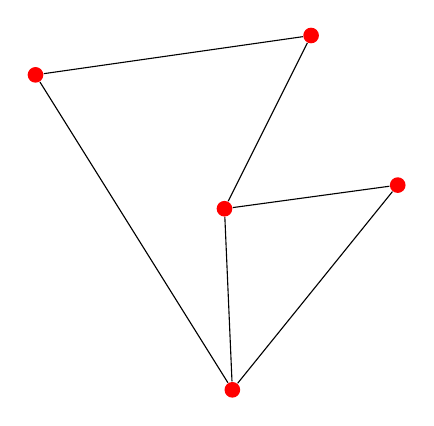
\begin{tikzpicture}

		% Nodes
		\node[fill=red, circle, inner sep=2pt, label=above:$a$] (a) at (0.4,0.3) {};
		\node[fill=red, circle, inner sep=2pt, label=above:$b$] (b) at (1.5,2.5) {};
		\node[fill=red, circle, inner sep=2pt, label=left:$c$] (c) at (-2,2) {};
		\node[fill=red, circle, inner sep=2pt, label=below:$d$] (d) at (0.5,-2) {};
		\node[fill=red, circle, inner sep=2pt, label=right:$e$] (e) at (2.6,0.6) {};

		% Edges
		\draw (a) -- (b);
		\draw (a) -- (d);
		\draw (a) -- (e);
		\draw (b) -- (c);
		\draw (c) -- (d);
		\draw (d) -- (e);

	\end{tikzpicture}
\end{minipage}
\begin{minipage}{0.4\textwidth}
	\[
		\begin{pmatrix}
			  & a & b & c & d & e \\
			a & 0 & 1 & 1 & 1 & 1 \\
			b & 1 & 0 & 1 & 0 & 0 \\
			c & 0 & 1 & 0 & 1 & 0 \\
			d & 1 & 0 & 1 & 0 & 1 \\
			e & 1 & 0 & 0 & 1 & 0 \\
		\end{pmatrix}
	\]
\end{minipage}
% \begin{figure}[H]
% 	\centering
% 	\includegraphics[width=0.8\textwidth]{matriz.png}
% 	\label{fig:matriz.png}
% \end{figure}

\begin{remark}
	Las matrices de adyacencias tambien se pueden utilizar para representar grafos no dirigidos con lazos y aristas multiples. Asi, un lazo en el vertice \(v_i \) viene representado por un \(1 \) en la posicion \(a_{ii}\) de la matriz de adyacencia. Si se trata de multigrafos, en la posicion \(a_{ij }\) de la matriz colocaremos el numero de aristas que conectan el vertice \(v_i \) y el \(v_j \). Asi, si tenemos 3 aristas entre el vertice \(v_i \) y el \(v_j ,\) pondremos \(a_{ij} = 3 \). En cualquier caso, todos los grafos no dirigidos tienen asociadas matrices simetricas.
\end{remark}

\begin{remark}
	En el caso de los grafos dirigidos la situacion es similar. En la posicion \(a_{ij }\) aparecera un 1 si hay una arista dirigida cuyo vertice inicial es \(v_i \) y cuyo vertice final es \(v_j \) y un cero en caso contrario. Observese que las matrices de adyacencias asociadas a grafos dirigidos no son necesariamente simetricas.
\end{remark}

Para dar un grafo basta con dar su matriz de adyacencia y muchas propiedades del grafo se pueden obtener directamente de propiedades de sus matrices de adyacencia, como por ejemplo:
\begin{itemize}
	\item El numero de vertices de un grafo es el numero de filas (o columnas) de sus matrices de adyacencia.
	\item El grado de un vertice es la suma de los elementos de la fila (o columna) correspondiente de la matriz de adyacencia.
	\item Un grafo es no dirigido si su matriz de adyacencia es simetrica.
	\item Un grafo contiene lazos si algun elemento de la diagonal de la matriz de adyacencia es no nulo.
	\item Un grafo tiene mas de una arista entre dos vertices si alguno de los elementos de su matriz de adyacencia es mayor que \(1 \).
	\item Si el grafo es no dirigido y no contiene lazos, usando el Teorema de Euler, el numero de aristas es la mitad de la suma de todos los elementos de su matriz de adyacencia.
	\item \dots
\end{itemize}

\vspace{0.3cm}
\section{Algunos grafos notables}
\begin{definition}
	Se denomina grafo completo de \(n \) vertices al grafo simple de \(n \) vertices \(K_n = (\set{1,2,\ldots,n}, \set{\set{i,j}; 1 \leq i < j \leq n })\). Esto significa que cada par de vertices distintos son adyacentes.
\end{definition}

\begin{proposition}
	El grafo completo \(K_n \) tiene las siguientes propiedades:
	\begin{itemize}
		\item El numero de vertices es \(n \)
		\item El grado de cada vertice es \(gr(v_1) = \cdots = gr(v_n) = n - 1\)
		\item El numero de aristas, usando el Teorema de Euler es
		      \[
			      |E| = \frac{1}{2} \sum_{i=1}^{n } gr(v_i ) = \frac{1}{2} \sum_{i=1}^{n } (n-1) = \frac{n(n-1)}{2}
		      \]
		\item Su matriz de adyacencia es
		      \[
			      \begin{pmatrix}
				      0      & 1      & 1      & \cdots & 1      \\
				      1      & 0      & 1      & \cdots & 1      \\
				      1      & 1      & 0      & \cdots & 1      \\
				      \cdots & \cdots & \cdots & \cdots & \cdots \\
				      1      & 1      & 1      & \cdots & 0      \\
			      \end{pmatrix}
		      \]
		      o equivalentemente \({\large{1}_{n \times n}} - I_n\).
	\end{itemize}
\end{proposition}

\begin{definition}[Grafo bipartido]
	Se dice que un grafo simple \(G = (V,E )\) es bipartido si su conjunto de vertices \(V \) se puede expresar como la unión de dos subconjuntos no vacios disjuntos \(V_1 \) y \(V_2\) de manera que cada arista del grafo conecta un vertice de \(V_1 \) con un vertice de \(V_2 \). Esto es, no existe una arista entre dos vertices de \(V_1 \) ni entre dos vertices de \(V_2 \): si \(\set{u,v} \in E \) entonces \(|\set{u,v} \cap V_i | = 1\), \(i = 1,2\).
\end{definition}
\begin{center}
	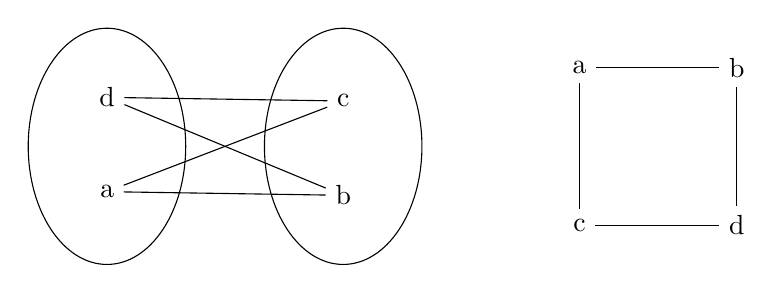
\begin{tikzpicture}
		% Draw the Venn diagram with nodes V1 and V2
		\draw (0,0) ellipse (1cm and 1.5cm) node (v1) at (0,0) {};
		\draw (3,0) ellipse (1cm and 1.5cm) node (v2) at (3,0) {};
		% \node[ellipse, draw, minimum width=2cm, minimum height=3cm, label=above:V1] (v1) at (0,0) {};
		% \node[ellipse, draw, minimum width=2cm, minimum height=3cm, label=above:V2] (v2) at (3,0) {};

		% Nodes in V1
		\node (a) at (v1.north) [below=5mm] {a};
		\node (d) at (v1.south) [above=5mm] {d};

		% Nodes in V2
		\node (b) at (v2.north) [below=5mm] {b};
		\node (c) at (v2.south) [above=5mm] {c};

		% Connecting lines
		\draw (a) -- (b);
		\draw (a) -- (c);
		\draw (d) -- (b);
		\draw (d) -- (c);

		% Draw the square graph
		\node (a2) at (6,1) {a};
		\node (b2) at (8,1) {b};
		\node (c2) at (6,-1) {c};
		\node (d2) at (8,-1) {d};

		% Draw edges
		\draw (a2) -- (b2);
		\draw (a2) -- (c2);
		\draw (b2) -- (d2);
		\draw (c2) -- (d2);
	\end{tikzpicture}
\end{center}

¿Cómo saber si un grafo es bipartido?
\begin{itemize}
	\item Si contiene un ciclo con una cantidad impar de vertices NO puede ser bipartido.
	\item Existe un algoritmo para saber si es bipartido o no que, en caso de que lo sea, nos da la bipartición del conjunto de vértices.
\end{itemize}

\begin{definition}[Grafo bipartido completo]
	Sea \(V_1 = \set{1,\ldots,m }\) y \(V_2 = \set{1^\prime,\ldots,n^\prime }\). El grafo bipartido completo \(K_{m,n} = (V,E )\) se define como \(V = V_1 \cup V_2 \) y \(E = \set{\set{j,k^\prime } \colon j \in V_1, k^\prime \in V_2 }\). Esto es, \(V \) se puede expresar como la union de dos subconjuntos disjuntos \(V_1 \) de \(m \) vertices y \(V_2 \) de \(n \) vertices, de manera que cada vertice de \(V_1 \) esta conectado con todos los vertices de \(V_2 \) y ninguna arista conecta un par de vertices de \(V_1 \) ni de \(V_2\).
\end{definition}
\begin{center}
	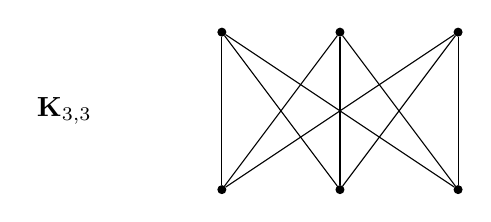
\begin{tikzpicture}
		% Title
		\node[align=center] at (-0.5, 0) {\textbf{K\(_{3,3}\)}};

		% Nodes
		\foreach \i in {1,2,3}
			{
				\node[draw, circle, fill, inner sep=1pt] (top\i) at (\i*1.5, 1) {};
				\node[draw, circle, fill, inner sep=1pt] (bottom\i) at (\i*1.5, -1) {};
			}

		% Edges
		\foreach \i in {1,2,3}
		\foreach \j in {1,2,3}
		\draw (top\i) -- (bottom\j);
	\end{tikzpicture}
\end{center}

\begin{itemize}
	\item En general los grafos bipartidos son diferentes de los grafos bipartidos completos.
\end{itemize}

\begin{example}
	Calcular el numero de vertices, grados, numero de aristas y matriz de adyacencia del grafo \(K_{n,m} (n,m \in \N )\)

	\begin{itemize}
		\item Numero de vertices: Si \(K_{n,m} = (V,E )\), entonces \(V = V_1 \cup V_2\) particion de \(V \) con \(V_1 \) conjunto de \(n \) vectores y \(V_2\) conjunto de \(m \) vectores \(\Rightarrow \) el numero de vertices es \(|V| = |V_1| + |V_2| = n + m \)
		\item Grado de los vertices: Si \(v \in V_1 \Rightarrow gr(v) = m \). Si \(v \in V_2 \Rightarrow gr(v) = n \).
		\item Numero de aristas: Usando el teorema de Euler, \(2|E| = \sum_{v \in V} gr(v) = \sum_{v \in V_1} gr(v) + \sum_{v \in V_2} gr(v) = m \cdot n + n \cdot m = 2 \cdot m \cdot n \Rightarrow |E| = n \cdot m   \)
		\item Matriz de adyacencia: Si denotamos \(V_1 = \set{v_1,\ldots,v_n}\) y \(V_2 = \set{w_1,\ldots,w_m}\).

		      Tomando el orden de vertices \(v_1,\ldots,v_n,w_1,\ldots,w_m \) la matriz de adyacencia es
		      \[
			      A = \begin{pmatrix}
				      0      & 0      & \cdots & 0      & 1      & \cdots & 1      \\
				      0      & 0      & \cdots & 0      & 1      & \cdots & 1      \\
				      \cdots & \cdots & \cdots & \cdots & \cdots & \cdots & \cdots \\
				      0      & 0      & \cdots & 0      & 1      & \cdots & 1      \\
				      1      & 1      & \cdots & 1      & 0      & \cdots & 0      \\
				      \cdots & \cdots & \cdots & \cdots & \cdots & \cdots & \cdots \\
				      1      & 1      & \cdots & 1      & 0      & \cdots & 0      \\
			      \end{pmatrix} =
			      \left ( \begin{array}[pos]{c|c}
					      0_{n\times n }  & 1_{n \times m } \\ \hline
					      1_{m \times n } & 0_{m \times m}  \\
				      \end{array} \right )
		      \]
	\end{itemize}
\end{example}

\section{Caminos y conexion}
\begin{definition}[Camino]
	Un camino de longitud \(n \) entre los vertices \(a \) y \(b \) de un grafo no dirigido es una sucesion finita \((e_0, \ldots, e_{n-1})\) de aristas del grafo
	\[
		e_0 = \set{v_{0}, v_1}, e_1 = \set{v_1,v_2},\ldots,e_{n-1} = \set{v_{n-1}, v_n },
	\]
	de manera que \(v_0 = a \), \(v_n = b \) y cada arista sucesiva empieza donde termino la anterior. Si el grafo es simple, el camino \((e_0, \ldots, e_{n-1})\) queda perfectamente determinado por la sucesion de vertices
	\[
		(a,v_1,v_2,\ldots,v_{n-1}, b ).
	\]
	Diremos que el camino anterior pasa por (o atraviesa) los vertices
	\(a\), \(v_1\), \(v_2\), \(\ldots\), \(v_{n-1}\), \(b \).

	Se dice que un camino es un circuito si es cerrada, esto es, empieza y termina en el mismo vertice, es decir, si \(a = b\).

	Se dice que un camino es simple si no contiene a la misma arista mas de una vez.

	Un circuito que no pasa dos veces por el mismo vertice (salvo el inicial por el que pasa dos veces) se llama ciclo.
\end{definition}

\begin{definition}[Conexo]
	Se dice que un grafo no dirigido \(G \) es conexo si para cualquier par de vertices \(a \) y \(b \) de \(G \) existe un camino entre \(a \) y \(b \).
\end{definition}

Si un grafo no es conexo, se puede expresar como la union de dos o mas subgrafos conexos de manera que los conjuntos de vertices y de aristas de cada par de estos subgrafos son disjuntos entre si. A estos subgrafos se les denomina componentes conexas del grafo dado. De esta manera un grafo es conexo si y solo si tiene una unica componente conexa.

\begin{theorem}
	Sea \(G \) un grafo (dirigido o no dirigido, con aristas multiples y lazos o no) y sea \(A = (a_{ij })\) su matriz de adyacencias con respecto al orden \(v_1,v_2,\ldots,v_{n-1},v_n \) de su conjunto de vertices. En estas condiciones el numero de caminos de longitud \(m \) entre el vertice \(v_i \) y el vertice \(v_j \) es igual al coeficiente situado en el lugar \((i,j )\) de la potencia \(m\)-esima de la matriz \(A \) (con respecto al producto de matrices usual).
\end{theorem}
\begin{proof}
	No la hacemos, pero se puede hacer por induccion sobre la longitud del camino entre dos vertices cualesquiera \(v_i \) y \(v_j \) de un grafo \(G \).
\end{proof}

\begin{corollary}
	Dado un grafo \(G = (V,E )\) tal que \(|V| = n \), se verifica que \(G \) es conexo si y solo si la matriz
	\[
		I_n + A + A^{2} + \cdots + A^{n-1}
	\]
	tiene todos los coeficientes distintos de cero.
\end{corollary}
\begin{example}
	Sea \(G \) un grafo cuya matriz de adyacencia es:
	\[
		A = \begin{pmatrix}
			0 & 1 & 0 \\
			1 & 0 & 1 \\
			0 & 1 & 0 \\
		\end{pmatrix}
	\]
	Entonces su cuadrado es
	\[
		A^{2} \coloneqq \begin{pmatrix}
			1 & 0 & 1 \\
			0 & 2 & 0 \\
			1 & 0 & 1 \\
		\end{pmatrix}
	\]
	Por tanto \(I_3 + A + A^{2 } \) tiene todas sus entradas no nulas y el grafo es conexo.
\end{example}

\begin{definition}[Camino euleriano]
	Un camino euleriano en un grafo no dirigido \(G \) es un camino simple que contiene a todas las aristas de \(G \). Un circuito euleriano en \(G \) es un circuito simple que contiene todas las aristas del grafo \(G \).
\end{definition}
\begin{definition}[Grafo euleriano]
	Se dice que un grafo no dirigido es euleriano si contiene un circuito euleriano.
\end{definition}

Un camino euleriano es un camino que recorre todas las aristas del grafo y sin repetir ninguna.

\begin{theorem}
	Un grafo \(G = (V,E )\) con aristas no dirigidas es euleriano si y solo si todas las aristas estan en la misma componente conexa y todos los vertices tienen grado par.
\end{theorem}
El siguiente resultado nos da una condicion para la existencia de un camino euleriano no cerrado:
\begin{proposition}
	Un grafo \(G = (V,E )\) con aristas no dirigidas tal que todas sus aristas estan en la misma componente conexa admite un camino euleriano no cerrado si y solo si contiene exactamente dos vertices de grado impar.
\end{proposition}

\begin{proposition}[Algoritmo de Fleury]
	Para calcular caminos/ciclos eulerianos en un grafo que los admite, usamos el algoritmo de Fleury:
	\begin{itemize}
		\item Comprobacion previa: Todas las aristas estan en la misma componente conexa y a lo sumo hay dos nodos de grado impar (necesario para que existan cambios eulerianos).
		\item Paso inicial: elegimos un vertice (\(v_0 \)) del siguiente modo:
		      \begin{itemize}
			      \item Si hay vertices de grado impar, elegimos uno de grado impar al azar.
			      \item Si no hay vertices de grado impar, elegimos uno de grado par al azar.
		      \end{itemize}
		\item Elegimos al azar una arista incidente en el vertice elegido en el paso anterior que no desconecte el grafo. Si no es posible hacerlo, elegimos una de las aristas incidentes al azar. En ambos casos borramos la arista elegida del grafo y nos movemos al vertice del otro extremo de la arista eliminada.
		\item Repetimos el proceso hasta que no queden aristas.
	\end{itemize}
	La sucesion de aristas construidas antes es un camino/ciclo euleriano.
\end{proposition}

\begin{definition}[Camino hamiltoniano]
	Se denomina camino hamiltoniano en un grafo con aristas no orientadas \(G = (V,E )\) a cualquier camino simple que contenga a todos los vertices de \(G \) pasadno una sola vez por cada uno de ellos, pero permitiendo que el vertice inicial de dicho camino sea igual al vertice final. Si el camino hamiltoniano es cerrado, a dicho camino se le denomina circuito hamiltoniano.
\end{definition}
\begin{definition}[Grafo hamiltoniano]
	Se dice que un grafo no dirigido \(G = (V,E )\) es hamiltoniano si contiene un circuito hamiltoniano.
\end{definition}
Pese a la aparente similitud con la definicion de los grafos eulerianos encontrar un circuito hamiltoniano en un grafo puede no ser tarea facil pues no se conoce una caracterizacion de los grafos hamiltonianos.

Como se ha comentado, no siempre es sencillo determinar si un grafo simple y conexo dado es hamiltoniano pues, para ello, el unico criterio que tenemos a priori es nuestra habilidad para encontrar o no un circuito hamiltoniano en el grafo dado. La siguiente proposicion nos aporta un resutlado que permite concluir que ciertos grafos son hamiltonianos.

\begin{theorem}[de Dirac]
	Sea \(G = (V,E )\) un grafo simple conexo de \(n \) vertices (\(n \geq 3 \)) tal que para cualquier vertice \(v \in V \) se cumple que
	\[
		gr(v) \geq \frac{n }{2 }.
	\]
	entonces \(G \) es hamiltoniano.
\end{theorem}

El Teorema de Dirac da una condicion suficiente para saber si un grafo es hamiltoniano, pero esta condicion no es una condicion necesaria (en general).

Hasta el momento no existe ninguna caracterizacion de los grafos hamiltonianos en terminos de los grados del grafo.

\begin{definition}[Isomorfismo de grafos]
	Se dice que dos grafos simples \(G_1 = (V_1,E_1 )\) y \(G_2 = (V_2,E_2 )\) son isomorfos si existe una biyeccion \(f \colon V_1 \to V_2 \) tal que \(\forall u,v \in V_1 \)
	\[
		\set{u,v} \in E_1 \iff \set{f(u),f(v)} \in E_2
	\]
	De la funcion \(f \) que satisface dicha condicion se dice que es un isomorfismo de grafos entre los grafos \(G_1 \) y \(G_2 \).
\end{definition}
En otras palabras, dos grafos simples son isomorfos si existe una funcion biyectiva entre los dos conjuntos de vertices que preserva las adyacencias. Naturalmente esta definicion se puede extender a multigrafos y multidigrafos teniendo en cuenta el numero de aristas entre cada par de vertices y, en su caso, la orientacion de las aristas.

\begin{example}
	Los dos grafos de la figura son isomorfos. Para verlo basta comprobar que la funcion \(f\colon \set{a,b,c,d} \to \set{u,v,w,p }\), tal que \(f(a) = u \), \(f(b) = v \), \(f(c) = w \), \(f(d) = p \) es un isomorfismo de grafos.

	\begin{center}
		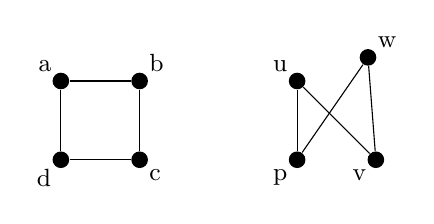
\begin{tikzpicture}
			% Define styles for the nodes and labels
			\tikzstyle{vertex} = [circle, fill=black, inner sep=0pt, minimum size=6pt]
			\tikzstyle{label} = [font=\small, anchor=east]

			% Define the nodes with positions
			\node[vertex] (a) at (0, 1) {};
			\node[vertex] (b) at (1, 1) {};
			\node[vertex] (c) at (1, 0) {};
			\node[vertex] (d) at (0, 0) {};

			\node[vertex] (u) at (3, 1) {};
			\node[vertex] (v) at (4, 0) {};
			\node[vertex] (w) at (3.9, 1.3) {};
			\node[vertex] (p) at (3, 0) {};

			% Draw the edges for the left graph
			\draw (a) -- (b);
			\draw (b) -- (c);
			\draw (c) -- (d);
			\draw (d) -- (a);

			% Draw the edges for the right graph
			\draw (u) -- (p);
			\draw (u) -- (v);
			\draw (p) -- (w);
			\draw (w) -- (v);

			% Place the labels
			\node[label, anchor=south east] at (a) {a};
			\node[label, anchor=south west] at (b) {b};
			\node[label, anchor=north west] at (c) {c};
			\node[label, anchor=north east] at (d) {d};

			\node[label, anchor=south east] at (u) {u};
			\node[label, anchor=north east] at (v) {v};
			\node[label, anchor=south west] at (w) {w};
			\node[label, anchor=north east] at (p) {p};

		\end{tikzpicture}
	\end{center}
\end{example}

A menudo es dificil determinar si dos grafos simples son isomorfos. De hecho, empleando herramientas de combinatoria, puede comprobarse que hay \(n! \) aplicaciones biyectivas entre los conjuntos de vertices de dos grafos con \(n \) vertices, por lo que comprobar una por una si dichas biyecciones preservan las adyacencias no es un buen metodo, sobre todo si \(n \) es un numero grande.

Debemos encontrar criterios para determinar si dos grafos simples son isomorfos o no lo son que no precisen una comprobacion exhaustiva.

Estos criterios se apoyan en el hecho de que hay ciertas propiedades, denominadas invariantes por isomorfismo, que, si un grafo las verifica, cualquier otro grafo isomorfo a el las debe tambien verificar. Por ejemplo:
\begin{enumerate}
	\item Dos grafos isomorfos deben tener el mismo numero de vertices y el mismo numero de aristas.
	\item Si \(f \colon V_1 \to V_2 \) establece un isomorfismo entre los grafos \(G_1 = (V_1, E_1 )\) y \(G_2 = (V_2, E_2 )\), entonces para cada \(u \in V_1 \) se tiene que \(gr(u) = gr(f(u ))\).
\end{enumerate}
Este tipo de resultados sirve para comprobar con cierta facilidad que algunos grafos no son isomorfos.

\begin{theorem}
	Si tenemos dos grafos que son isomorfos, entonces comparten todos los invariantes.

	Por tanto, si tenemos dos grafos que no comporten algun invariante, entonces no pueden ser isomorfos.
\end{theorem}
